% ---------------------------------------------------------------
% Preamble
% ---------------------------------------------------------------
%\documentclass[a4paper,fleqn,longmktitle]{cas-sc}
\documentclass[a4paper,fleqn]{cas-dc}
%\documentclass[a4paper]{cas-dc}
%\documentclass[a4paper]{cas-sc}
% ---------------------------------------------------------------
% Make margins bigger to fit annotations. Use 1, 2 and 3. TO be removed later
%\paperwidth=\dimexpr \paperwidth + 6cm\relax
%\oddsidemargin=\dimexpr\oddsidemargin + 3cm\relax
%\evensidemargin=\dimexpr\evensidemargin + 3cm\relax
%\marginparwidth=\dimexpr \marginparwidth + 3cm\relax
% -------------------------------------------------------------------- 
% Packages
\usepackage[switch]{lineno}
\linenumbers

% --------------------------------------------------------------------
% Figure packages
\usepackage{graphicx,float}
\usepackage{adjustbox}
% Text, input, formatting, and language-related packages
\usepackage[T1]{fontenc}
\usepackage{subcaption}

\usepackage{nomencl}
\makenomenclature

\usepackage{etoolbox}
\renewcommand\nomgroup[1]{%
	\item[\bfseries
	\ifstrequal{#1}{A}{}{%
		\ifstrequal{#1}{B}{Greek symbols}{%
			\ifstrequal{#1}{C}{Abberivations}{
	}}}%
	]}
\newcommand{\nomunit}[1]{%
	\renewcommand{\nomentryend}{\hspace*{\fill}#1}}


% TODO package
\usepackage[bordercolor=gray!20,backgroundcolor=blue!10,linecolor=black,textsize=footnotesize,textwidth=1in]{todonotes}
\setlength{\marginparwidth}{1in}
% \usepackage[utf8]{inputenc}
% \usepackage[nomath]{lmodern}

% Margin and formatting specifications
%\usepackage[authoryear]{natbib}
\usepackage[sort]{natbib}
\setcitestyle{square,numbers}

%\bibliographystyle{cas-model2-names}

\usepackage{setspace}
\usepackage{subfiles} % Best loaded last in the preamble

% \usepackage[authoryear,longnamesfirst]{natbib}

% Math packages
\usepackage{amsmath, amsthm, amssymb, amsfonts, bm, nccmath, mathdots, mathtools, bigints, ulem}

\usepackage{tikz}
\usepackage{pgfplots}
\usetikzlibrary{shapes.geometric,angles,quotes,calc}

\usepackage{placeins}

\usepackage[final]{pdfpages}

% --------------------------------------------------------------------
% Packages Configurations
\usepackage{enumitem}
% --------------------------------------------------------------------
% (General) General configurations and fixes
\AtBeginDocument{\setlength{\FullWidth}{\textwidth}}	% Solves els-cas caption positioning issue
\setlength{\parindent}{20pt}
%\doublespacing
% --------------------------------------------------------------------
% Other Definitions
% --------------------------------------------------------------------
\graphicspath{{Figures/}}
% --------------------------------------------------------------------
% Environments
% --------------------------------------------------------------------
% ...

% --------------------------------------------------------------------
% Commands
% --------------------------------------------------------------------

% ==============================================================
% ========================== DOCUMENT ==========================
% ==============================================================
\begin{document} 
	%  --------------------------------------------------------------------
	
	% ===================================================
	% METADATA
	% ===================================================
	\title[mode=title]{Local sensitivity analysis of a supercritical extraction model}                      
	\shorttitle{Sensitivity analysis}
	
	\shortauthors{OS, PO}
	
	\author[1]{Oliwer Sliczniuk}[orcid=0000-0003-2593-5956]
	\ead{oliwer.sliczniuk@aalto.fi}
	\cormark[1]
	\credit{a}
	
	\author[1]{Pekka Oinas}[orcid=0000-0002-0183-5558]
	\credit{b}
	
	%\author[1]{Francesco Corona}[orcid=0000-0002-3615-1359]
	%\credit{c}
	
	\address[1]{Aalto University, School of Chemical Engineering, Espoo, 02150, Finland}
	%\address[2]{2}
	
	\cortext[cor1]{Corresponding author}
	
	% ===================================================
	% ABSTRACT
	% ===================================================
	\begin{abstract}
	This study investigates the process of chamomile oil extraction from chamomile flowers. A parameter-distributed model, consisting of a set of partial differential equations, was used to describe the governing mass transfer phenomena between solid and fluid phases under supercritical conditions using carbon dioxide as the solvent. The concept of quasi-one-dimensional flow was applied to reduce the number of spatial dimensions. The flow of carbon dioxide is assumed to be uniform across any cross-section, although the area available for the fluid phase can vary along the extractor. The physical properties of the solvent were estimated using the Peng-Robinson equation of state. Laboratory experiments were conducted under various, but constant operating conditions of $30 - 40~^\circ C$, $100 - 200$ bar and $3.33-6.67 \cdot 10^{-5}$ kg/s. The local sensitivity analysis method was applied to evaluate the robustness of the model parameters by investigating the impact of infinitesimally small changes in the model parameters and controls on the model outputs. This study focuses on analysing the effect of pressure on the model state space and extraction yield. It was found that the model is the most sensitive to the controls if operated close to the critical point.
		
	\end{abstract}
	
	\begin{keywords}
		supercritical extraction \sep sensitivity analysis \sep mathematical modelling
	\end{keywords}
	
	% ===================================================
	% TITLE
	% ===================================================
	\maketitle
	
	% ===================================================
	% Section: Introduction
	% ===================================================
	
	\section{Introduction}
	
	%\subfile{Sections/introduction_imp}
	Supercritical CO$_2$ is defined as carbon dioxide that is pressurized and heated above its critical point (31.1 $^\circ C$, 74 bar). Depending on the operating conditions, the fluid properties such as viscosity and density can vary, which leads to multiple industrial applications of CO$_2$.
	
	One of the most popular applications of supercritical CO$_2$ is the extraction of essential oils, as described by many researchers, for example, by \citet{Sodeifian2017}, \citet{Reverchon1993}, or \citet{Sovova1994}. Traditional methods, such as distillation and organic solvent extraction, are commonly employed but have drawbacks. Distillation involves high temperatures that can lead to the thermal degradation of heat-sensitive compounds. This limitation has increased the popularity of alternative techniques, such as supercritical fluid extraction. Supercritical CO$_2$ is appealing due to its distinctive properties: it is inflammable, non-toxic, and non-corrosive. Supercritical fluids can exhibit both gas- and liquid-like properties, allowing for adjustable dissolving power through changes in operating conditions.
	
	The applications of supercritical carbon dioxide are not limited only to an extraction process but can also be used for impregnation, as described by \citet{Weidner2018} and \citet{Machado2022} Impregnation is defined as modifying the properties of bulk substances by physically or chemically binding/adsorbing impregnates to a bulk material or surface, such as the hydrophobization of surfaces. The main advantage of using supercritical CO$_2$ is that, after depressurization, it desorbs from the surface and evaporates, leaving a solvent-free product. On the other hand, the main disadvantage of using carbon dioxide for impregnation is the low solubility of many drugs of interest.
	The study by \citet{Ameri2020} investigates the loading of lansoprazole into polymers using supercritical carbon dioxide and examines how various parameters, such as temperature, pressure, and time, affect the drug loading efficiency. The results indicate that increasing any of these parameters enhances drug loading, with temperature having the most significant impact. \citet{Fathi2022} explored the use of supercritical carbon dioxide to enhance the bioavailability of ketoconazole by impregnating it into water-soluble polymers, specifically polyvinylpyrrolidone and hydroxypropyl methylcellulose. Utilizing a Box--Behnken design, the researchers optimized the impregnation process by varying pressure, temperature, and time, achieving increase in drug loadings ranging.
	
	Another application of supercritical CO$_2$ is nanoparticle formation, as investigated by \citet{Padrela2018}, \citet{Franco2021}, and \citet{Sodeifian2022} Supercritical carbon dioxide-assisted technologies enable the production of different morphologies of different sizes, including nanoparticles and nanocrystals, by modulating the operating conditions. Supercritical fluid-based processes have advantages over techniques conventionally employed to produce nanosized particles or crystals, such as reduced use of toxic solvents. Moreover, the CO$_2$ is removed from the final product by simple depressurization. 
	\citet{Sodeifian2018} investigated the solubility of Letrozole, a poorly water-soluble anticancer drug, in supercritical carbon dioxide with and without menthol as a solid co-solvent. The addition of menthol increased Letrozole's solubility by 7.1 times compared to supercritical CO$_2$ alone. Using the rapid expansion of supercritical solutions with solid co-solvent method, the average particle size of Letrozole was reduced to the nanoscale. Temperature was found to have the most significant impact on nanoparticle size reduction, while pressure had the least effect. 
	The study of \citet{SaadatiArdestani2020} explored the preparation of phthalocyanine green nano pigment using supercritical carbon dioxide as an antisolvent. The researchers employed the gas antisolvent technique to achieve nano-sized particles of the pigment.
	\citet{Sodeifian2019} analyzed the production of amiodarone hydrochloride nanoparticles using an ultrasonic-assisted rapid expansion of supercritical solution into a liquid solvent method. By optimizing parameters such as pressure, temperature, and polymeric stabilizer concentration, the researchers achieved significant particle size reduction. Characterization techniques confirmed the successful formation of nanoparticles with improved properties.
	
	This study investigates the extraction of essential oil from chamomile flowers (Matricaria chamomilla L.) via supercritical fluid extraction techniques and the modelling of this process. Chamomile is a medicinal herb widely cultivated in southern and eastern Europe---in countries such as Germany, Hungary, France and Russia. It can also be found outside Europe, for instance in Brazil, as discussed by \citet{Singh2011} This plant is distinguished by its hollow, bright gold cones, housing disc or tubular florets and surrounded by about fifteen white ray or ligulate florets. Chamomile has been used for its medicinal benefits, serving as an anti-inflammatory, antioxidant, mild astringent, and healing remedy. Extracts of chamomile are widely used to calm nerves and mitigate anxiety, hysteria, nightmares, insomnia and other sleep-related conditions, according to \citet{Srivastava2009}. \citet{Orav2010} reported that oil yields from dried chamomile samples ranged from 0.7 to 6.7 mL/kg. The highest yields of essential oil, between 6.1 and 6.7 mL/kg, were derived from chamomile sourced from Latvia and Ukraine. In comparison, chamomile from Armenia exhibited a lower oil content of 0.7 mL/kg.
	
	The literature offers various mathematical models to describe the extraction of valuable compounds from biomass. Selecting a process model is case-dependent and requires analysis of each model's specific assumptions about mass transfer and thermodynamic equilibrium.
	
	Depending on the needs, one of two approaches can be considered while developing a mathematical model for the extraction process. A model which is based on a multiple regression can be used if the relation between inputs and outputs is the only one of interest. \citet{Sodeifian2017a} investigated the influence of pressure, temperature, and particle size on the extraction efficiency of oil from dracocephalum kotschyi boiss seed. The second order polynomial model was applied to obtain the corresponding response surface and to identify the optimum operating conditions. 
	The study of \citet{Sodeifian2017b} investigates the of essential oil from Eryngium billardieri, focusing on optimizing extraction conditions and developing a mathematical model based on the second order polynomial to predict the process yield. The researchers employed a simulated annealing algorithm to optimize parameters such as pressure, temperature, and extraction time, aiming to maximize oil efficiency.
	
	Alternatively, a first principle model can be derived and applied to cover not only the input--output relations, but the phenomena occurring in the system. This approach allows for more detailed representation the system behaviour, but requires deeper understanding of the underlying physics and more rigorous experiments.
	
	\citet{Goto1996} presented the shrinking core (SC) model, which describes a process of irreversible desorption that is followed by diffusion through the pores of a porous solid. When the mass transfer rate of the solute in the non-extracted inner region is significantly slower than in the outer region, where most of the solute has already been extracted or when the solute concentration exceeds its solubility in the solvent, a distinct boundary may form between the inner and outer regions. As extraction progresses, the core of the inner region shrinks. The model envisions supercritical CO$_2$ extraction as a sharp, inward-moving front, with a completely non-extracted core ahead of the front and a fully extracted shell behind it.
	
	\citet{Sovova1994} proposed the broken-and-intact cell (BIC) model, which assumes that a portion of the solute, initially stored within plant structures and protected by cell walls, is released during the mechanical breakdown of the material. The solute located in the region of broken cells near the particle surface is directly exposed to the solvent, while the core of the particle contains intact cells with undamaged walls. This model describes three extraction phases: a fast extraction phase for accessible oil, a transient phase, and a slow phase controlled by diffusion. The model has been successfully applied to the extraction of grape oil (\citet{Sovova1994b}) and caraway oil (\citet{Sovova1994a}).
	
	The supercritical fluid extraction (SFE) process can be treated similarly to heat transfer, considering solid particles as hot balls cooling down in a uniform environment. \citet{Bartle1990} introduced the hot ball diffusion (HBD) model, where spherical particles with a uniformly distributed solute diffuse similarly to heat diffusion. Unlike the BIC model, where the solute is readily available on the particle surface, the HBD model is suited for systems with small quantities of extractable materials and is not limited by solubility. The model is particularly relevant when internal diffusion controls mass transfer, allowing results from single particles to be extended to the entire bed under uniform conditions. \citet{Reverchon1993} have further elaborated on the HBD model and used it to simulate extraction processes.
	
	\citet{Reverchon1996} proposed a model for extraction of essential oils, which are mainly located inside the vegetable cells in organules called vacuoles. Only a small fraction of essential oil might be near the particle surface due to the breaking up of cells during grinding or in epidermal hairs located on the leaf surface. The fraction of oil freely available on the particle surface should not be significant in the case of SFE from leaves. Consequently, SFE of essential oil from leaves should be mainly controlled by internal mass-transfer resistance. Therefore, the external mass-transfer coefficient was neglected in the development of the model of \citet{Reverchon1996}. The mass balances were developed with the additional hypotheses that axial dispersion can be neglected and that the solvent density and flow rate are constant along the bed.
	
	This work builds upon the linear kinetic model suggested by \citet{Reverchon1996}, deriving fundamental governing equations to develop a comprehensive model for the chamomile oil extraction process. This model aims at control-oriented simplicity, assuming semi-continuous operation within a cylindrical vessel. The process involves a supercritical solvent being pumped through a fixed bed of finely chopped biomass to extract the solute, followed by separation of the solvent and solute in a flush drum to collect the extract. Parameters such as pressure ($P$), feed flow rate ($F$), and inlet temperature ($T_{in}$) are adjustable and measurable, while the outlet temperature ($T_{out}$) and the amount of product at the outlet can only be monitored. Figure \ref{fig: SFE_drawing} presents a simplified process flow diagram.
	
	\begin{figure}[h!]
		\centering
		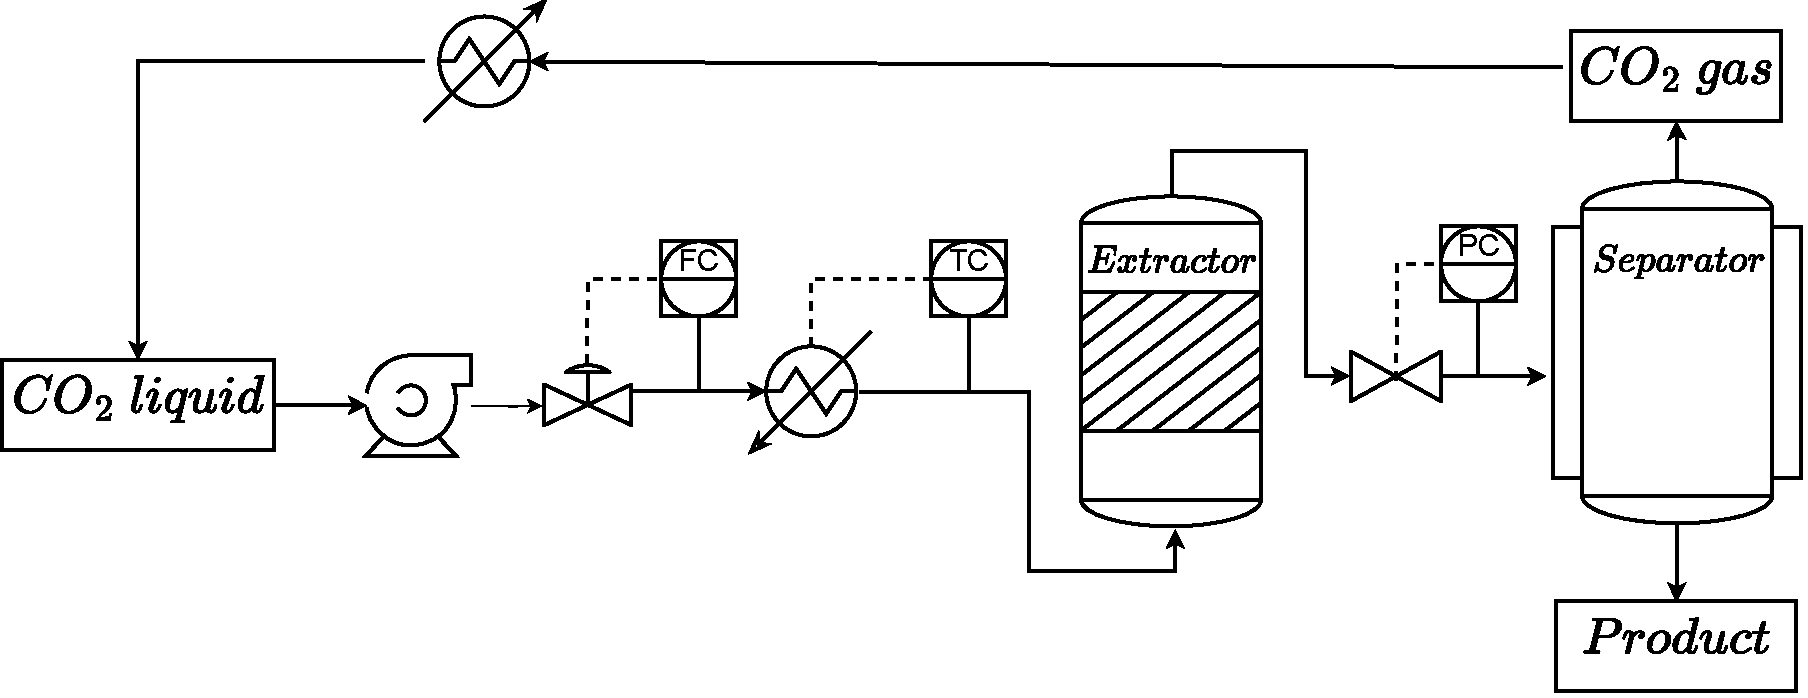
\includegraphics[width=\columnwidth]{Figures/PFD.drawio.pdf}
		\caption{Process flow diagram.}
		\label{fig: SFE_drawing}
	\end{figure}
	
	The primary aim of this study is to analyze the influence of changes in operating conditions on the process model developed by \citet{Sliczniuk2024}. Understanding how variations in parameters and control variables affect the model's behaviour is essential for improving its accuracy, robustness, and practical applicability. To achieve this, a comprehensive sensitivity analysis is employed, serving as a systematic approach to assess the impact of model parameters and controls on the outputs. The results of this sensitivity analysis are valuable for multiple purposes. First, they help identify sources of uncertainty within the model, highlighting which parameters most significantly influence predictions. Second, they provide insights for potential model simplification, allowing the exclusion of non-essential parameters without compromising accuracy. Finally, the analysis can detect inconsistencies or errors by uncovering unexpected relationships between inputs and outputs, which may signal flaws in the model's assumptions or structure.
	
	A range of sensitivity analysis methods can be utilized to achieve these objectives, including:
	
	\begin{itemize}
		\item One-at-a-time method
		\item Derivative-based local methods
		\item Variance-based methods
	\end{itemize}
	
	Different supercritical extraction models have been analyzed using various sensitivity analysis techniques in the literature. For instance, \citet{Fiori2007} performed sensitivity calculations by varying parameters within their confidence intervals and observing the changes in model results. Their analysis revealed that the particle diameter and internal mass transfer coefficient significantly influence extraction during the diffusion-control regime.
	
	\citet{Santos2000} considered the model of \citet{Sovova1994} for semi-continuous isothermal and isobaric extraction processes using carbon dioxide as a solvent. They conducted a parametric sensitivity analysis using a two-level factorial design, disturbing model parameters by 10\% and analyzing their main effects. They proposed strategies for high-performance operation based on sensitivities related to superficial velocity, particle diameter, initial solute concentration in the solid phase, and solute concentration in the fluid phase at the extractor inlet.
	
	\citet{Hatami2024} performed a one-factor-at-a-time sensitivity analysis to assess the response of net present value (NPV) to variations in technical and economic variables. Their study consisted of two parts. The first part examined how net present value is influenced by changes in individual technical and economic parameters, keeping the extractor volume constant at 300 L. The second part investigated the effects of varying the extractor volume (from 1 to 600 L) on the project's profitability. The authors found that the raw material price, discount rate and residence time had the biggest impact on NPV.
	
	The study by \citet{Maly1996} addressed the development of numerical methods and software tools for sensitivity analysis in differential-algebraic equation systems. It thoroughly examines the mathematical foundations of the local sensitivity analysis methods employed, providing an in-depth analysis of their performance. The authors presented a variety of problems to demonstrate the efficiency and applicability of their approach.
		
	In another work, \citet{Turanyi1990} presented a comprehensive review of sensitivity analysis methods for spatially homogeneous, constant-parameter chemical kinetic systems. This study explored a range of sensitivity analysis techniques, including concentration sensitivity, rate sensitivity, and feature sensitivity analysis. Practical applications of these methods in chemical kinetics were highlighted, showcasing their utility in understanding and predicting system behaviour.
		
	\citet{Fishtik1997} applied local sensitivity analysis to a complex chemical reaction system involving multiple pure condensed phases and one ideal gas phase. The study demonstrated that the system's response could be expressed as a sum of contributions from equilibrium states defined by gas-phase species. The impact of temperature, pressure, and initial species amounts was specifically analyzed in the context of coal gasification.
		
	In their comprehensive review, \citet{Saltelli2005} examined sensitivity analysis methods applicable to chemical reaction modelling. They discussed both local and global techniques, emphasizing the role of global sensitivity analysis in understanding complex chemical systems. The authors highlighted the importance of variance-based methods in quantifying the influence of input parameters on model outputs by discussing results of a few simulation analysis.
	
	A key novelty of this work lies in its rigorous application of derivative-based local sensitivity analysis to a first-principles model of supercritical fluid extraction. While multiple publications available in the literature discuss application of sensitivity analysis on a supercritical extraction model, many of these either omit local sensitivity analyses and focus on basic parametric comparisons (\citet{Santos2000}, \citet{Fiori_2007}, or \citet{Zahedi2010}). In contrast, the present approach integrates a quasi-1D partial-differential-equation model with automatic differentiation of the mass and energy balances, enabling a detailed exploration of how infinitesimal changes in parameters, which propagates propagate through the system. As the result, corresponding system response of the state space (with emphasis on solutes concentrations on solid and liquid phase as well as yield). Although this work focus on the influence of a few selected parameters, the same methodology can be extended to any other parameter. Notably, this level of detail is crucial near the critical region of CO$_2$, where small deviations in process conditions can trigger large changes in solvent properties (such as density and solubility). This approach thus provides a systematic and quantitative measure of the system’s sensitivity to parameter fluctuations across different extraction regimes, from kinetic- to diffusion-controlled.
	
	% ===================================================
	% Section: Main
	% ===================================================
	
	%\subfile{Sections/Model}
	\section{Materials and methods} \label{CH: Materials and methods}
	
	\subsection{Governing equations} \label{CH:Governing_equations_chapter}
	The governing equations for a quasi-one-dimensional flow were derived following the work of \citet{Anderson1995}. A quasi-one-dimensional flow refers to a fluid flow scenario assuming that the flow properties are uniformly distributed across any cross-section. This simplification is typically applied when the flow channel's cross-sectional area changes, such as through irregular shapes or partial filling of an extractor. According to this assumption, velocity and other flow properties change solely in the flow direction.
	
	As discussed by \citet{Anderson2023}, all flows are compressible, but some of them can be treated as incompressible since the velocities are low. This assumption leads to the incompressible condition: $\nabla \cdot u =0$, which is valid for constant density (strict incompressible) or varying density flow. The assumption allows for removing acoustic waves and large perturbations in density and/or temperature. In the 1-D case, the incompressibility condition becomes $\frac{du}{dz} = 0$, so the fluid velocity is constant along the $z-$ direction.
	
	The set of quasi-one-dimensional governing equations in Cartesian coordinates is described by Equations \ref{EQ: CompressibleEuler_1}--\ref{EQ: CompressibleEuler_3}:
	
	{\footnotesize
		\begin{align}
			\label{EQ: CompressibleEuler_1}
			\cfrac{\partial \left( \rho_f A_f \right) }{\partial t} + \cfrac{\partial \left( \rho_f A_f v \right)}{\partial z} &= 0, \\
			\cfrac{\partial \left( \rho_f v A_f \right) }{\partial t} + \cfrac{\partial \left( \rho_f A_f v^2 \right)}{\partial z} &= -A_f \cfrac{\partial P}{\partial z} \label{EQ: CompressibleEuler_2}, \\
			\cfrac{\partial \left( \rho_f e A_f \right) }{\partial t} + \cfrac{\partial \left( \rho_f A_f v e\right)}{\partial z} &= -P\cfrac{\left( A_f v \right)}{\partial z} + \cfrac{\partial}{\partial z} \left( k \cfrac{\partial T}{\partial z} \right),   
			\label{EQ: CompressibleEuler_3}
		\end{align}  
	}
	
	where $\rho_f$ is the density of the fluid, $A_f$ is the function which describes a change in the cross-section, $v$ is the velocity, $P$ is the total pressure, $e$ is the internal energy of the fluid, $t$ is time, and $z$ is the spatial direction.
	
	\subsection{Extraction model} \label{CH: Extraction_model}
	\subsubsection{Continuity equation} \label{CH: Continuity}
	
	The previously derived quasi-one-dimensional continuity equation (Equation \ref{EQ: CompressibleEuler_1}) is redefined by incorporating the function $A_f = A\phi$. This modification distinguishes constant and varying terms, where the varying term accounts for changes in the cross-sectional area available for the fluid. Equation \ref{EQ: Continuity_differential} shows the modified continuity equation:
	
	{\footnotesize
		\begin{equation} \label{EQ: Continuity_differential}
			\frac{\partial (\rho_f \phi)}{\partial t} + \frac{\partial (\rho_f v A\phi)}{\partial z} = 0,
		\end{equation}
	}
	where $A$ is the total cross-section of the extractor and $\phi$ describes porosity along the extractor.
	
	Assuming that the mass flow rate is constant in time, the temporal derivative becomes the mass flux F, and the spatial derivative can be integrated along $z$ as follows:
	
	{\footnotesize
		\begin{equation}
			\int \frac{\partial (\rho_f v A \phi )}{\partial z} dz = F \rightarrow F=\rho_f v A\phi
		\end{equation}
	}
	
	To simplify the system dynamics, it is assumed that $F$ is a control variable and affects the whole system instantaneously (due to $\nabla \cdot u = 0$), which allows finding the velocity profile that satisfies mass continuity based on $F$, $\phi$, and $\rho_f$:
	
	{\footnotesize
		\begin{equation} \label{EQ:Velocity_1}
			v = \cfrac{F}{\rho_f A\phi} 
		\end{equation}
	}
	
	Similarly, superficial velocity may be introduced:
	
	{\footnotesize
		\begin{equation} \label{EQ:Velocity_2}
			u = v \phi = \cfrac{F}{\rho_f A }
		\end{equation}
	}
	
	The fluid density $\rho_f$ can be obtained from the Peng--Robinson equation of state if the temperature and thermodynamic pressure are known along $z$. Variation in fluid density may occur due to pressure or inlet temperature changes. In a non-isothermal case, in Equations \ref{EQ:Velocity_1} and \ref{EQ:Velocity_2}, $\rho_f$ is considered the average fluid density along the extraction column.
	
	\subsubsection{Mass balance for the fluid phase} \label{CH: Mass_balance_fluid}
	
	Equation \ref{Model_fluid} describes the movement of the solute in the system, which is constrained to the axial direction due to the quasi-one-dimensional assumption. Given that the solute concentration in the solvent is negligible, the fluid phase is described as pseudo-homogeneous, with properties identical to those of the solvent itself. It is also assumed that the thermodynamic pressure remains constant throughout the device. The analysis further simplifies the flow dynamics by disregarding the boundary layer near the extractor's inner wall. This leads to a uniform velocity profile across any cross-section perpendicular to the axial direction. Thus, the mass balance equation includes convection, diffusion and kinetic terms representing the fluid phase behaviour:
	
	{\footnotesize
		\begin{equation}
			\label{Model_fluid}
			\frac{\partial c_f}{\partial t}
			+ \frac{1}{\phi} \frac{\partial \left( c_f u\right)}{\partial z}
			= \frac{1-\phi}{\phi} r_e
			+ \frac{1}{\phi} \frac{\partial}{\partial z} \left( D^M_e \frac{\partial c_f}{\partial z} \right),
		\end{equation}
	}
	
	where $c_f$ represents the solute concentration in the fluid phase, $r_e$ is the mass transfer kinetic term and $D^M_e$ is the axial dispersion coefficient.
	
	\subsubsection{Mass balance for the solid phase} \label{Mass_balance_solid}
	
	As given by Equation \ref{Model_solid}, the solid phase is considered stationary, without convection and diffusion terms in the mass balance equation. Therefore, the only significant term in this equation is the kinetic term of Equation \ref{Model_kinetic_basic}, which connects the solid and fluid phases. For simplicity, the extract is represented by a single pseudo-component: 
	
	{\footnotesize
		\begin{equation} 
			\label{Model_solid}
			\cfrac{\partial c_s}{\partial t} = \underbrace{-r_e}_{\text{Kinetics}}
	\end{equation} }
	
	\subsubsection{Kinetic term} \label{CH: Kinetic}
	
	As the solvent flows through the fixed bed, CO$_2$ molecules diffuse into the pores, adsorb on the inner surface, and form a film due to solvent--solid matrix interactions. The dissolved solute diffuses into the bulk from the particle's core through the solid--fluid interface, the pore and the film. Figure \ref{fig: SFE_Mechanism} shows the mass transfer mechanism, where the mean solute concentration in the solid phase is denoted by $c_s$, and the equilibrium concentrations at the solid--fluid interface are denoted by $c_s^*$ and $c_p^*$ for the solid and fluid phases, respectively. The concentration of the solutes in the fluid phase in the centre of the pore is denoted by $c_p$. As the solute diffuses through the pore, its concentration changes, reaching $c_{pf}$ at the opening. Then, the solute diffuses through the film around the particle and reaches bulk concentration $c_f$. The two-film theory describes the solid-fluid interface inside the pore. The overall mass transfer coefficient can be determined from the relationship between the solute concentration in one phase and its equilibrium concentration.
	
	\begin{figure}[h!]
		\centering
		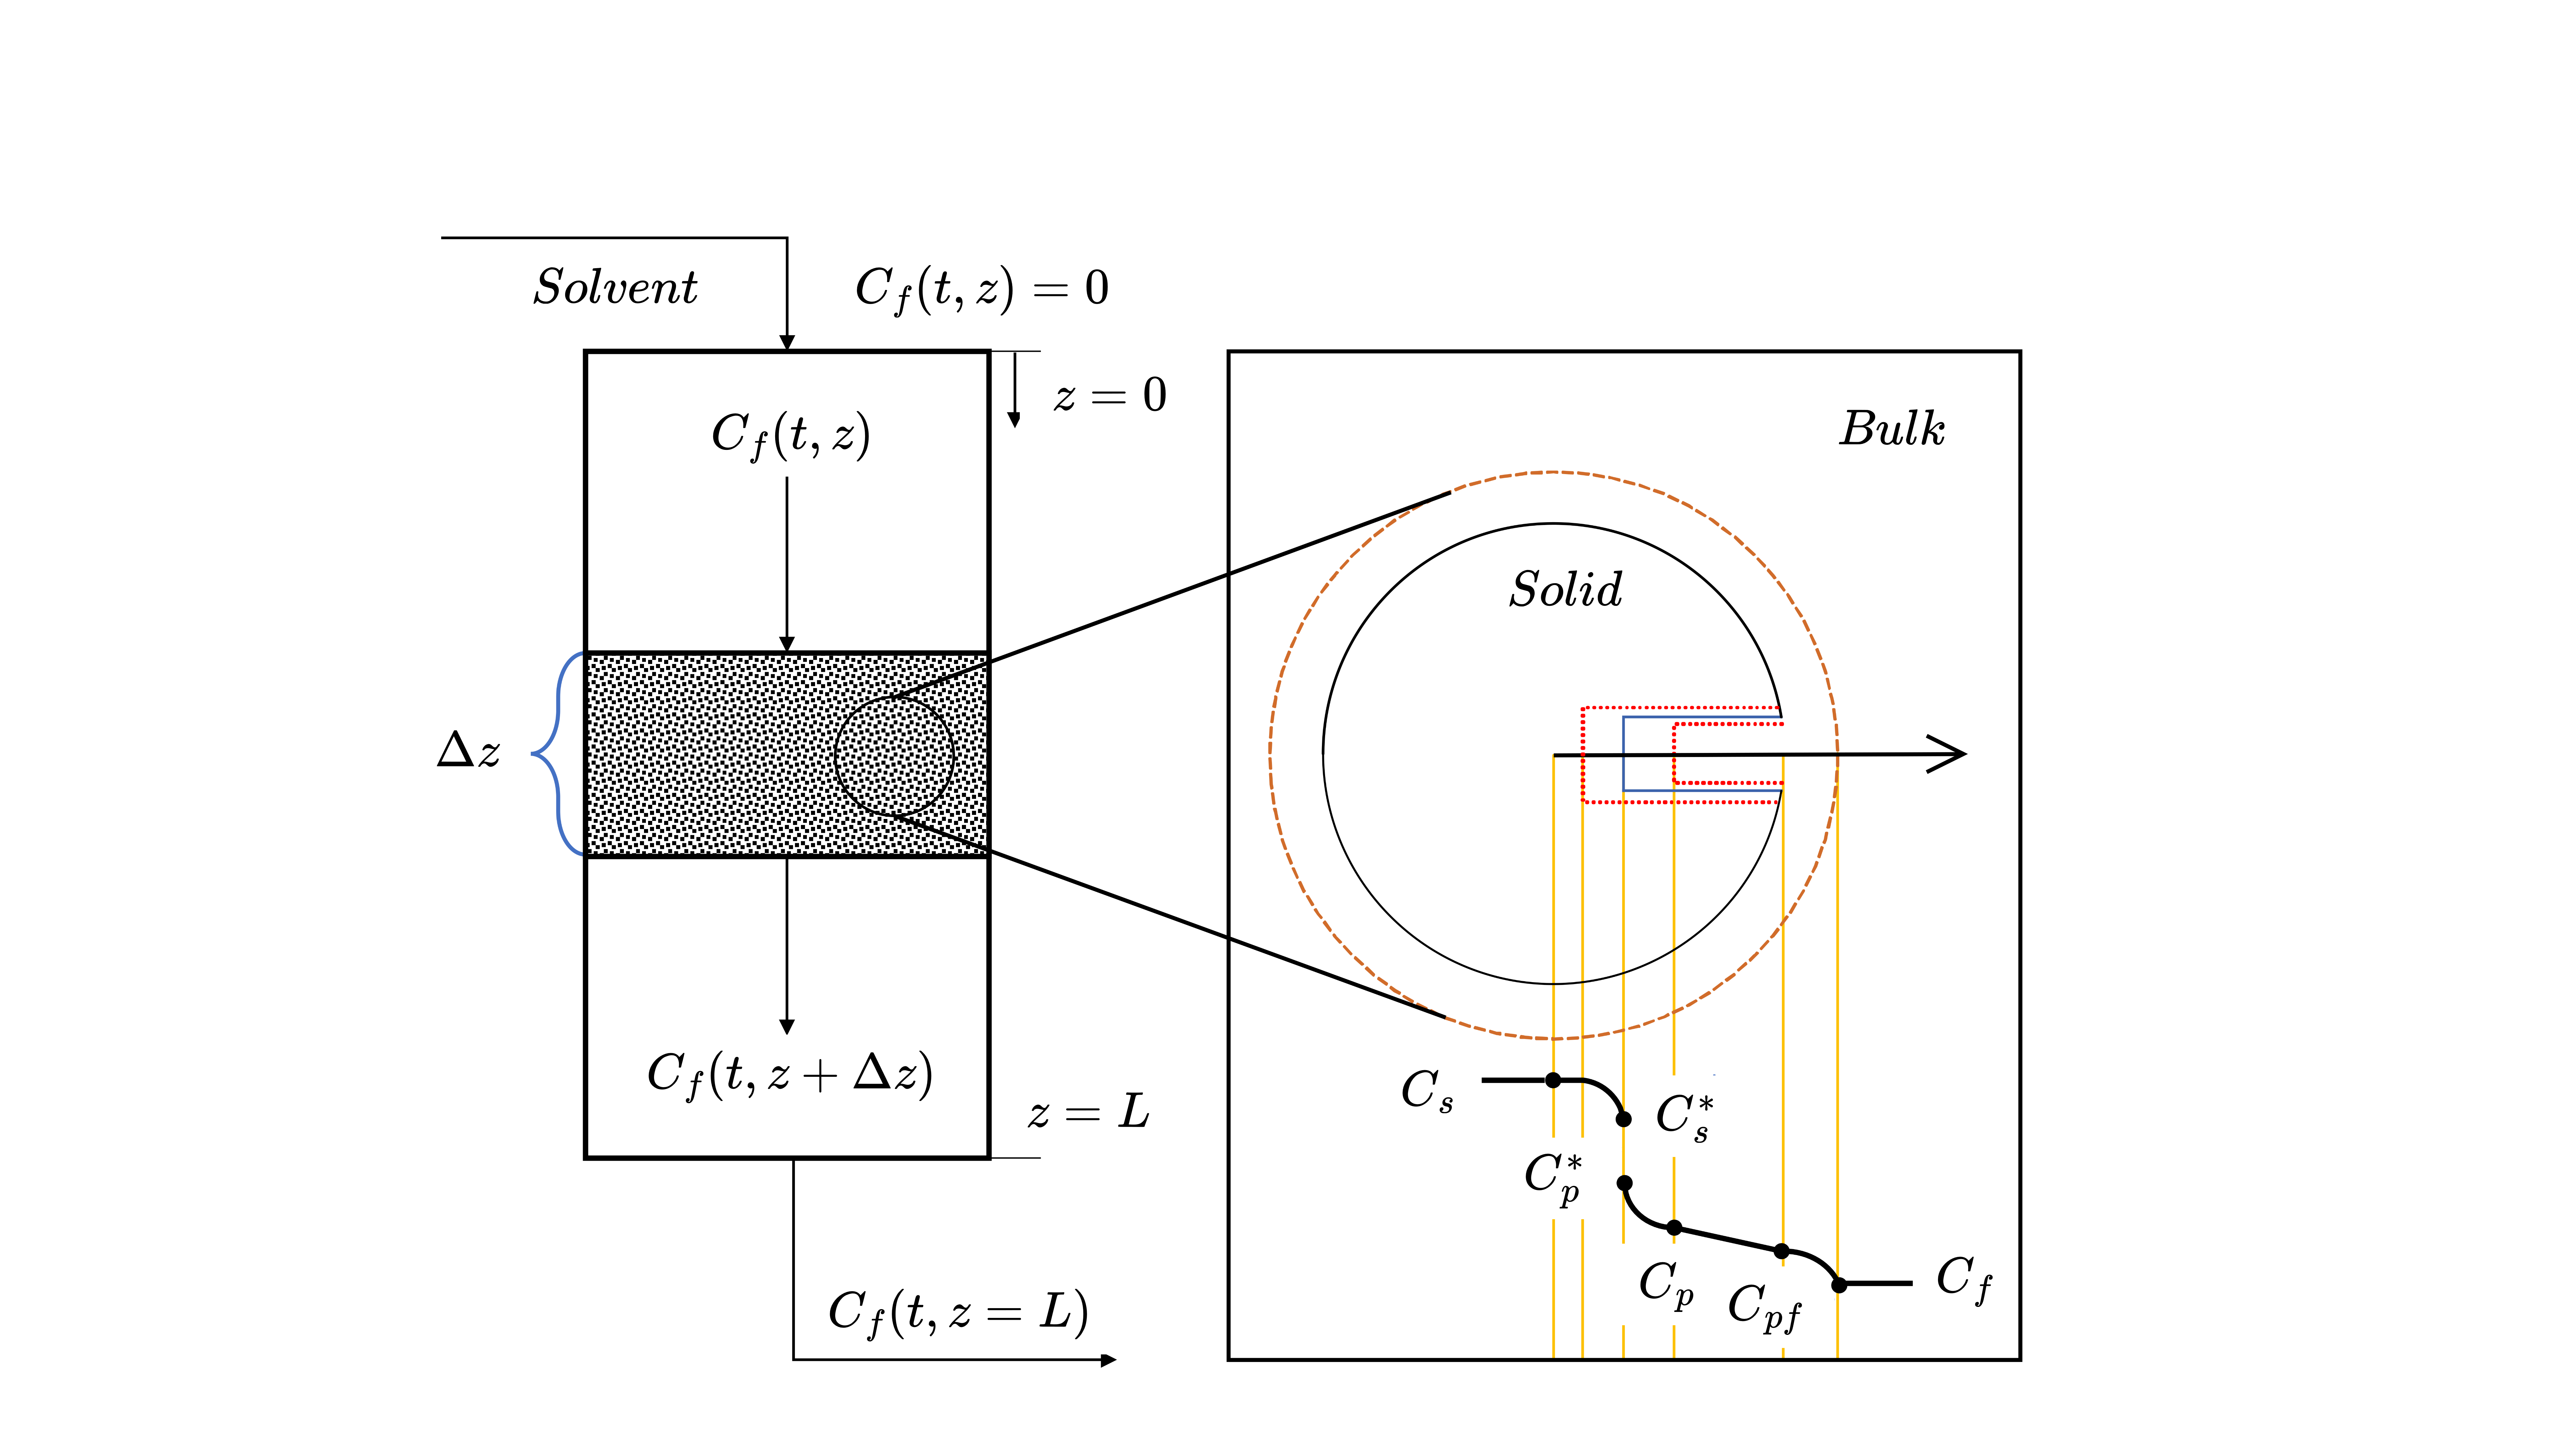
\includegraphics[trim = 45cm 0cm 60cm 20cm,clip,width=0.85\columnwidth]{Figures/SFE_PFD.drawio.png}	
		\caption{Mass transfer mechanism.}
		\label{fig: SFE_Mechanism}
	\end{figure}
	
	\citet{Bulley1984} suggest a process where the driving force for extraction is given by the difference between the concentration of the solute in the bulk, $c_f$, and in the centre of the pore, $c_p^*$. The concentration $c_p^*$ is in equilibrium with $c_s$ according to the equilibrium relationship. The rate of extraction is thus $r_e\left(c_f - c^*_p(c_s)\right)$. In contrast, \citet{Reverchon1996} proposes a driving force given by the difference between $c_s$ and $c_p^*$. As given in Equation \ref{Model_kinetic_basic}, the concentration $c_p^*$ is determined by the equilibrium relationship with $c_f$:
	
	{\footnotesize
		\begin{equation} \label{Model_kinetic_basic}
			r_e = \cfrac{D_i}{\mu l^2 }\left(c_s - c_p^* \right),
	\end{equation} }
	
	where $\mu$ is sphericity, $l$ a characteristic dimension of particles that can be defined as $l = r/3$, $r$ is the mean particle radius, $\rho_s$ is the solid density, $D_i$ corresponds to the overall diffusion coefficient, and $c_P^*$ is the concentration at the solid--fluid interface (which, according to the internal resistance model, is supposed to be at equilibrium with the fluid phase). 
	
	According to \citet{Bulley1984}, a linear equilibrium relationship (Equation \ref{Linear_equilibirum}) can be used to find the equilibrium concentration of the solute in the fluid phase $c_f^*$ based on the concentration of the solute in the solid phase $c_s$:
	
	{\footnotesize
		\begin{align} \label{Linear_equilibirum}
			c_f^* &= k_p c_s
	\end{align} }
	
	The volumetric partition coefficient $k_p$ acts as an equilibrium constant between the solute concentration in one phase and the corresponding equilibrium concentration at the solid--fluid interphase. \citet{Spiro2007} propose defining the mass partition coefficient $k_m$ as follows: 
	
	{\footnotesize
		\begin{align}
			k_m = \cfrac{k_p \rho_s}{\rho_f}
	\end{align} }
	
	According to \citet{Reverchon1996}, the kinetic term becomes the following:
	
	{\footnotesize
		\begin{equation}
			\label{Model_kinetic_no_sat}
			r_e = \cfrac{D_i}{ \mu l^2 } \left(c_s - \cfrac{\rho_s c_f}{k_m \rho_f} \right)
	\end{equation} }

	The choice between the two formulations should consider the system's properties and the underlying mass transfer assumptions. In systems where external mass transfer dominates, the resistance to solute transport primarily occurs at the fluid--solid interface, typically governed by the diffusion of solute across the fluid boundary layer. Under these conditions, the Bulley formulation is more appropriate, as it explicitly emphasizes the fluid-phase concentration ($c_f$) as the driving force for mass transfer through the term $c_f - c_p^*(c_s)$. Conversely, when internal mass transfer dominates, the resistance to solute transport is controlled by diffusion or adsorption processes within the solid phase. In such cases, the Reverchon formulation is more suitable, as it accounts for deviations in the equilibrium through the term $c_s - c_s^*(c_f)$.
	
	\subsubsection{Uneven distribution of solute in the solid phase} \label{CH: Gamma_Function}
	
	Following the idea of the broken-and-intact cell (BIC) model of \citet{Sovova2017}, the internal diffusion coefficient $D_i$ is considered to be a product of the reference value of $D_i^R$ and the exponential decay function $\gamma$, as given by Equation \ref{EQ: C_sat_function}:
	
	{\footnotesize
		\begin{equation}
			D_i = D_i^R \gamma(c_s) = D_i^R \exp \left( - \Upsilon \left( 1-\cfrac{ c_s }{c_{s0}} \right) \right), \label{EQ: C_sat_function}
	\end{equation} }
	
	where  $\Upsilon$ describes the curvature of the decay function. Equation \ref{Model_kinetic} describes the final form of the kinetic term:
	
	{\footnotesize
		\begin{equation}
			\label{Model_kinetic}
			r_e = \cfrac{D_i^R \gamma }{ \mu l^2 } \left( c_s  - \cfrac{\rho_s c_f }{ k_m \rho_f }  \right)
	\end{equation} }
	
	The $\gamma$ function limits the solute's availability in the solid phase. Similarly to the BIC model, the solute is assumed to be contained in the cells, some of which are open because the cell walls were broken by grinding, with the rest remaining intact. The diffusion of the solute from a particle's core takes more time than the diffusion of the solute close to the outer surface. The same idea can be represented by the decaying internal diffusion coefficient, where the decreasing term is a function of the solute concentration in the solid. 
	
	An alternative interpretation of the decay function $\gamma$ involves considering the porous structure of the solid particles, where the pores are initially saturated with the solute. During extraction, the solute within these pores gradually dissolves into the surrounding fluid. Initially, the solute molecules near the pore openings dissolve and diffuse rapidly due to the short diffusion paths. As the extraction progresses, the dissolution front moves deeper into the pore structure, and solute from the inner regions of the pores begins to dissolve. The diffusion of solute molecules from the interior of the pores to the external fluid becomes progressively slower because the effective diffusion path length increases. This lengthening of the diffusion path enhances the mass transfer resistance, reducing the overall diffusion rate. 
	
	In an extreme case, this model could be compared with the shrinking core model presented by \citet{Goto1996}, where the particle radius decreases as the solute content in the solid phase diminishes. In the SC model, the reduction in particle size leads to significant changes in both the diffusion path length and the surface area available for mass transfer. The diminishing particle size increases the diffusion path within the remaining solid core and decreases the external surface area, both of which contribute to a slower extraction rate. When comparing this to the varying diffusion coefficient in our model, some conceptual similarities can be noticed.
	
	\subsubsection{Empirical correlations}
	
	The empirical correlations for $D_i$ and $\Upsilon$ were derived by \citet{Sliczniuk2024} and validated for temperatures of $30 - 40^\circ C$, pressures of $100 - 200$ bar, and mass flow rates of $3.33-6.67 \cdot 10^{-5}$ kg/s. Figures \ref{fig:Correlation_Di} and \ref{fig:Correlation_Gamma} show the results of multiple linear regression applied to solutions of parameter estimation and selected independent variables. The region marked with the white dashed line represents the confidence region, where the model has been tested. Both correlations should be equal or greater than zero to avoid unphysical behaviour such as  reverse mass transfer. The multiple linear regression functions are combined with the rectifier function to ensure non-negativity.
	
	\begin{figure}[!ht]
		\centering
		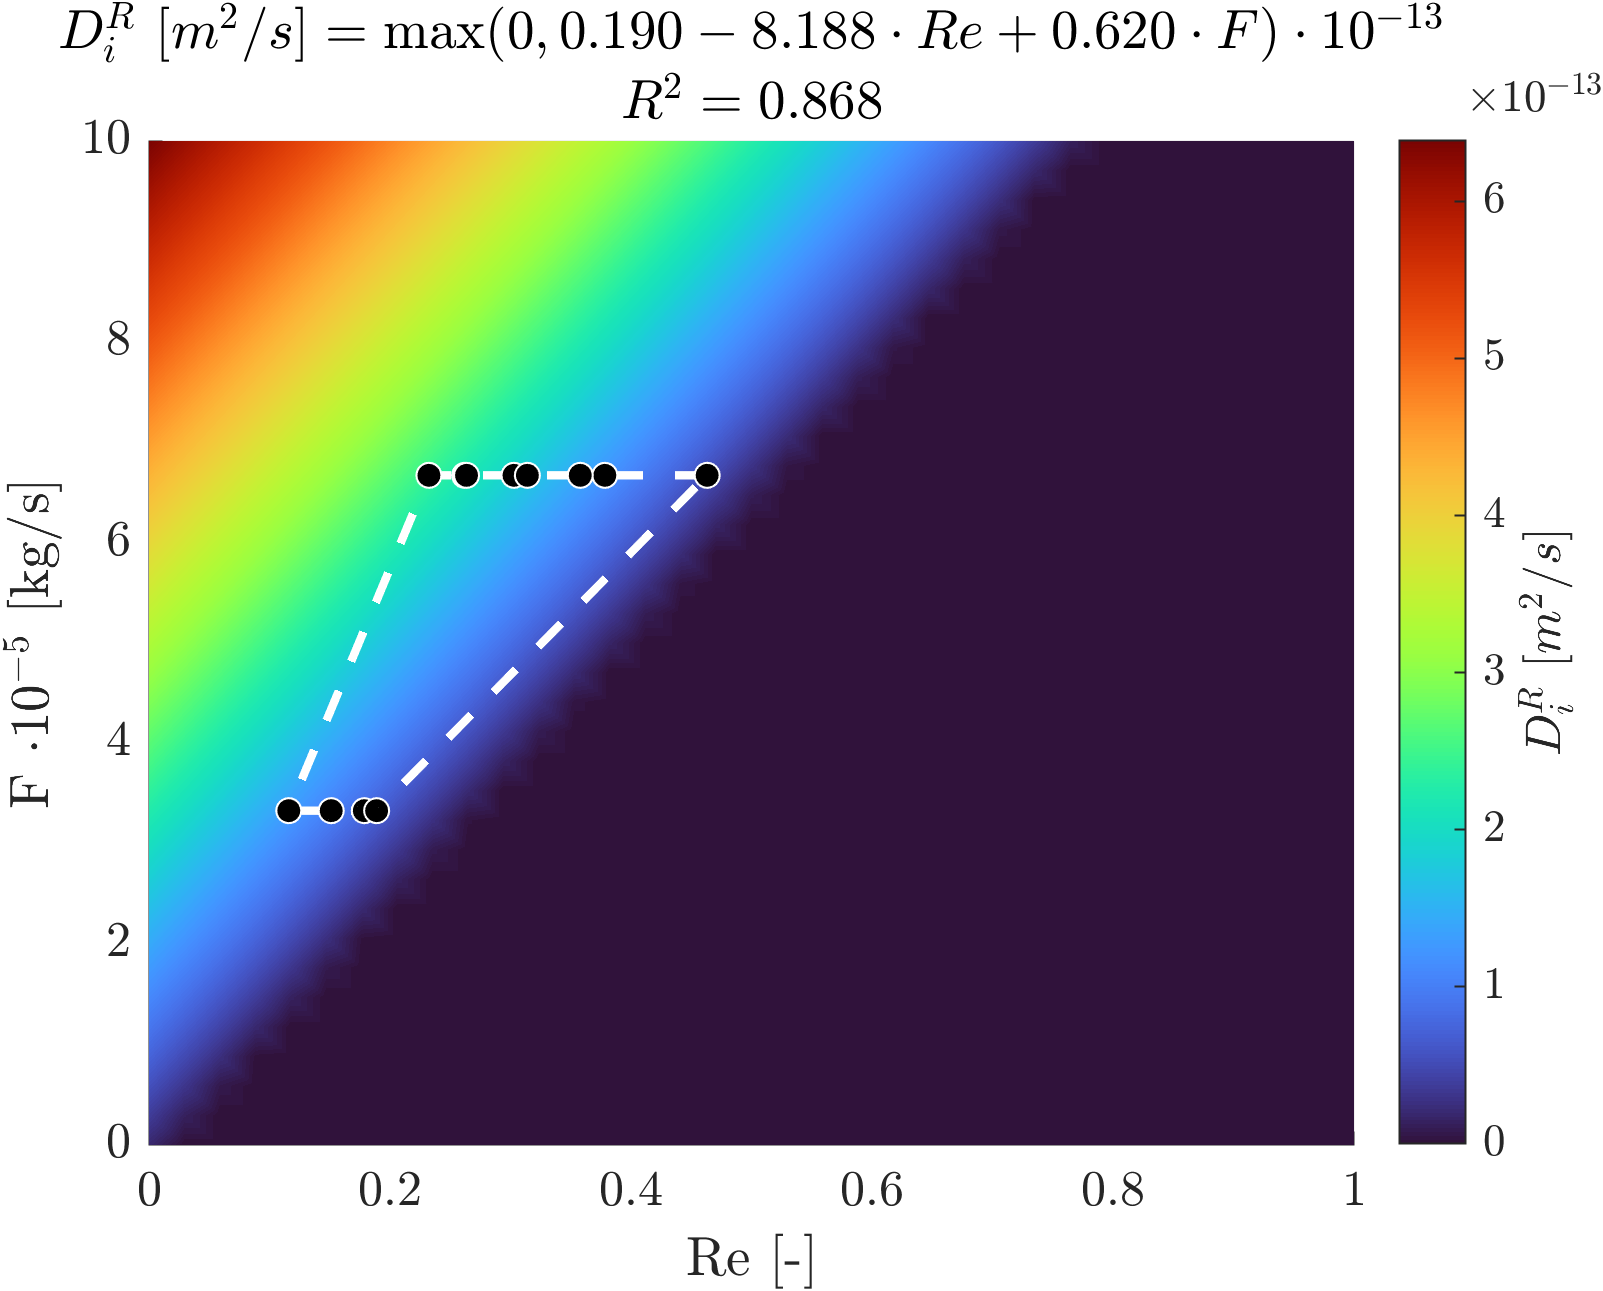
\includegraphics[trim = 0.0cm 0.0cm 0.0cm 0.0cm,clip,width=\columnwidth]{/Di.png}
		\caption{Multiple linear regression $D_i^R = f(Re, F).$}
		\label{fig:Correlation_Di}
	\end{figure}
	
	\begin{figure}[!ht]
		\centering
		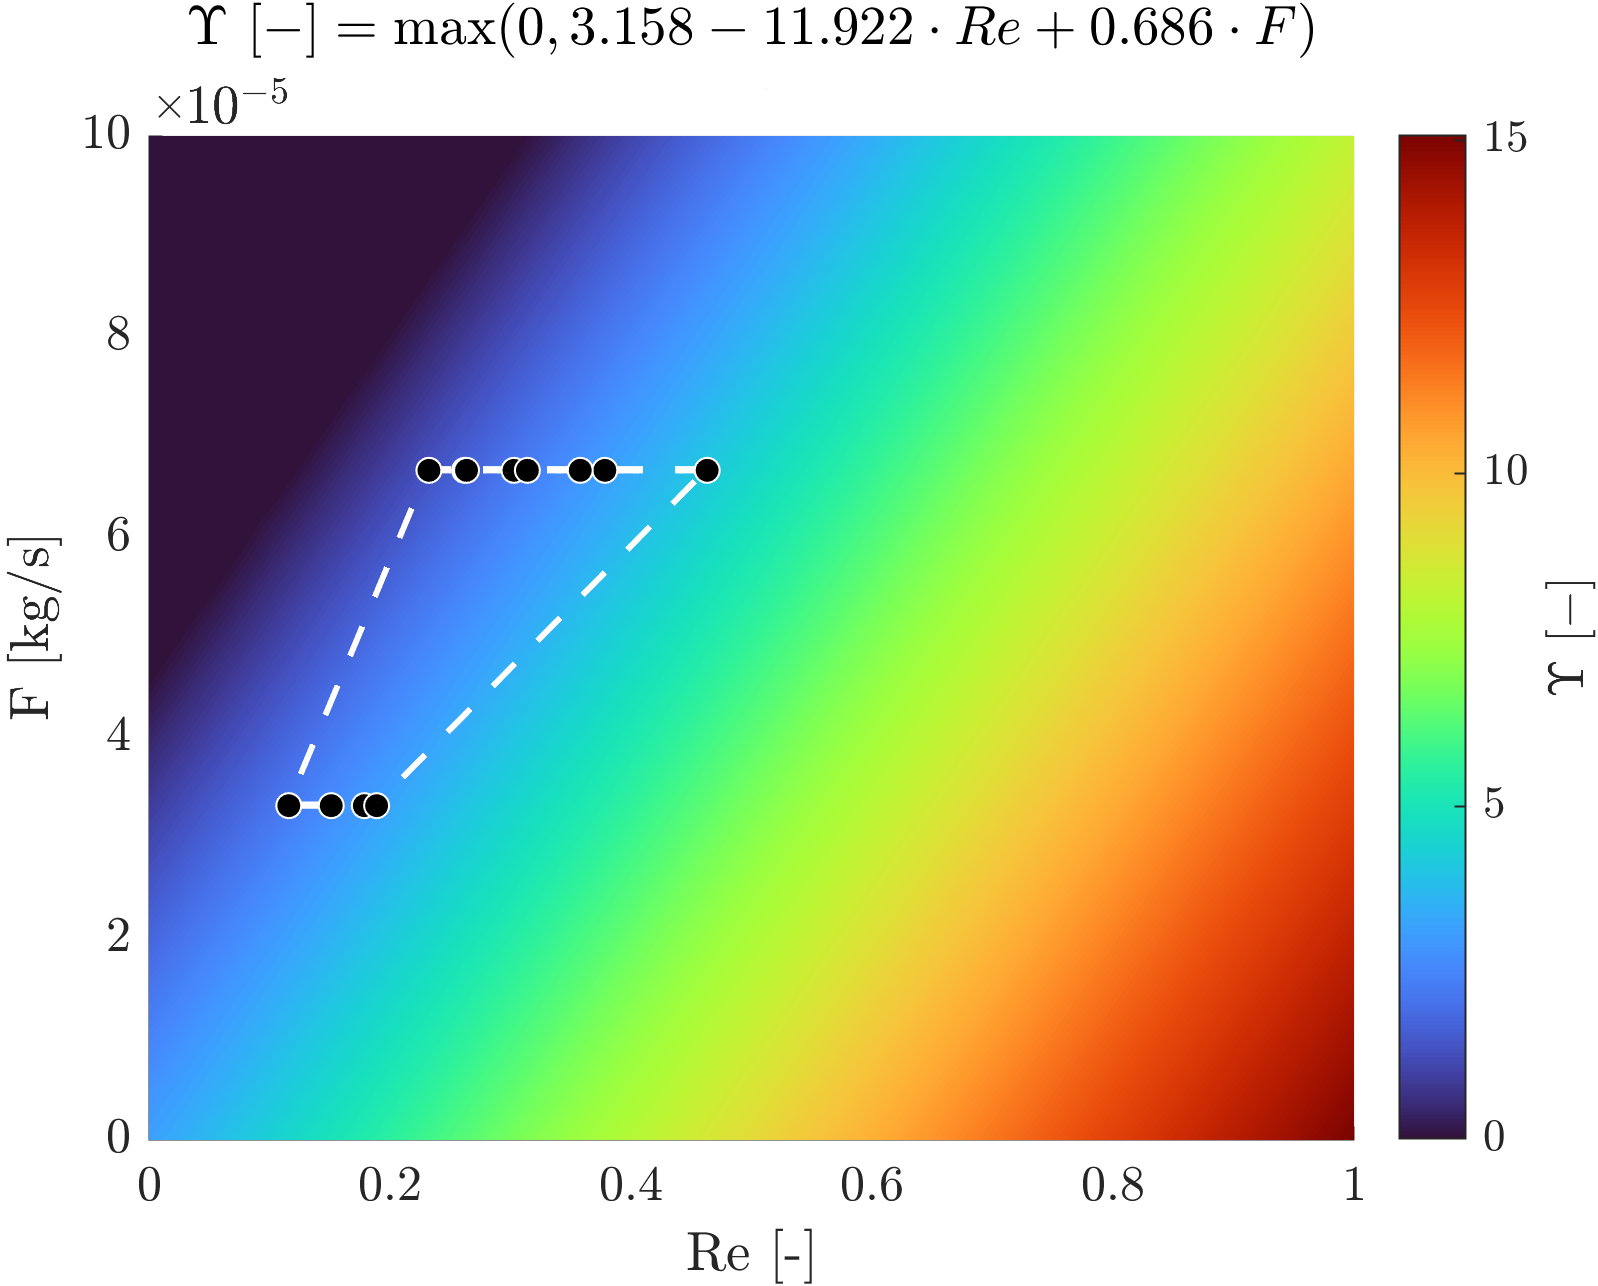
\includegraphics[trim = 0.0cm 0.0cm 0.0cm 0.0cm,clip,width=\columnwidth]{/Gamma.png}
		\caption{Multiple linear regression $\Upsilon = f(Re, F).$}
		\label{fig:Correlation_Gamma}
	\end{figure}
	
	\subsubsection{Heat balance} \label{CH: heat_balance}
	
	The heat balance equation describes the evolution of the enthalpy in the system and is given by Equation \ref{EQ:Enthalpy_equation}:
	
	{\footnotesize
		\begin{equation} \label{EQ:Enthalpy_equation}
			\cfrac{\partial \left(\rho_f h A_f\right)}{\partial t} = - \cfrac{\partial \left( \rho_f h A_f v \right)}{\partial z} + \cfrac{\partial \left(P A_f\right)}{\partial t} + \cfrac{\partial}{\partial z} \left( k \cfrac{\partial T}{\partial z} \right)
		\end{equation}
	}
	
	If the value of enthalpy $h$ is known from the time evolution of the energy equation, and pressure $P$ is known from measurement, then temperature $T$ can be reconstructed based on the departure function. The departure function is a mathematical function that characterizes the deviation of a thermodynamic property (enthalpy, entropy, or internal energy) of a real substance from that of an ideal gas at the same temperature and pressure. The enthalpy departure function, as presented by \citet{Gmehling2019} for the Peng--Robinson equation of state,  is defined by Equation \ref{EQ:Enthalpy_PR}:
	
	{\scriptsize
		\begin{equation}
			h-h^{id}=RT \left[T_r(Z-1) -2.078(1+\kappa ){\sqrt { \alpha\left(T\right) } } \ln \left(\cfrac{Z+\left( 1+\sqrt{2} \right)B}{Z+\left( 1-\sqrt{2} \right)B}\right)\right]
			\label{EQ:Enthalpy_PR}
		\end{equation}				
	}
	
	where $\alpha$ is defined as $\left( 1+\kappa \left( 1 - \sqrt{T_r} \right) \right)^2$, $T_r$ is the reduced temperature, $P_r$ is the reduced pressure, $Z$ is the compressibility factor, $\kappa$ is a quadratic function of the acentric factor, and $B$ is calculated as $0.07780\frac{P_r}{T_r}$.
	
	Equation \ref{EQ:Enthalpy_PR} requires a reference state, which is assumed to be $T_{ref}=298.15$ K and $P_{ref}=1.01325$ bar.
	
	A root finder can be used to find a temperature value which minimizes the difference between the value of enthalpy coming from the heat balance and the departure functions. The root-finding procedure has to be repeated at every time step to find a temperature profile along spatial direction $z$.
	
	{\footnotesize
		\begin{equation}
			\min_T \left( \underbrace{h\left(t,x\right)}_{\text{Heat balance}} - \underbrace{h\left(T,P,\rho_f\left(T,P\right)\right)}_{\text{Departure function}} \right)^2
			\label{EQ:Enthalpy_root}
		\end{equation}
	}
	
	\subsubsection{Pressure term} \label{CH: Pressure}
	
	As explained in Section \ref{CH:Governing_equations_chapter}, the pressure in the low-velocity region remains nearly constant due to the small pressure wave propagation occurring at the speed of sound. Under such conditions, the term $\partial P/\partial t$ can be approximated by a forward difference equation, describing the pressure change over a small time step $\Delta t$. The pressure $P$ in the system is treated as a state variable, while the incoming pressure at the new time-step $P_{in}$ is treated as a control:
	
	{\footnotesize
		\begin{equation}
			\frac{\partial P}{\partial t} \approx \frac{P_{in} - P }{\Delta t}
	\end{equation}}
	
	Such a simplified equation allows for instantaneous pressure. In a real system, the pressure dynamics would depend on the behaviour of the pump and the back-pressure regulator, which introduce additional inertia and resistance to pressure changes, leading to pressure gradual build-up.
	
	\subsubsection{Extraction yield} \label{CH: Yield}
	
	The process yield is calculated according to Equation \ref{Model_measurment_1}, as presented by \citet{Sovova1994a}. The measurement equation evaluates the solute's mass at the extraction unit outlet and sums it up. The integral form of the measurement (Equation \ref{Model_measurment_1}) can be transformed into the differential form (Equation \ref{Model_measurment_2}) and augmented with the process model.
	
	{\footnotesize
		\begin{align} 
			\label{Model_measurment_1}
			y &= \int_{t_0}^{t_f} \cfrac{F}{\rho_f} c_f \biggr\rvert_{z=L} dt \\
			\cfrac{dy}{dt} &= \qquad \cfrac{F}{\rho_f} c_f \biggr\rvert_{z=L} 
			\label{Model_measurment_2}
	\end{align}	}
	
	\subsubsection{Initial and boundary conditions} 
	It is assumed that the solvent is free of solute at the beginning of the process $c_{f0}=0$, that all the solid particles have the same initial solute content $c_{s0}$ and that the system is isothermal, hence the initial state is $h_0$. The fluid at the inlet is considered not to contain any solute. The initial and boundary conditions are defined as follows:
	
	{\footnotesize
		\begin{align*}
			&c_f(t = 0, z) = 0  && c_s(t = 0, z) = c_{s0} && h(t = 0, z) = h_0 \\
			&c_f(t,   z=0) = 0  && h(t, z=0) = h_{in}  && \frac{\partial c_f(t,z=L)}{\partial x} = 0 \\
			&\frac{\partial h(t,z=L)}{\partial x} = 0   && c_s(t, z=\{0,L\}) = 0 && y(0) = 0 \quad P(0) = P_0 \\
	\end{align*} }
	
	\subsubsection{Discretization methods}
	
	\begin{figure}[!h]
		\centering
		{\footnotesize
			\begin{align*}
				\dot{x} &= \cfrac{d x}{d t} = 
				\begin{bmatrix}
					\cfrac{d c_{f,1}}{d t} 	  \\
					\vdots					  \\
					\cfrac{d c_{f,N_z}}{d t} \\
					\\ \hline \\
					\cfrac{d c_{s,1}}{d t} 	  \\
					\vdots					  \\
					\cfrac{d c_{s,N_z}}{d t} \\
					\\ \hline \\
					\cfrac{d h_1}{d t} 	  \\
					\vdots 					  \\
					\cfrac{d h_{N_z}}{d t} \\
					\\ \hline \\
					\cfrac{d P}{d t} \\
					\\ \hline \\
					\cfrac{d y}{d t}
				\end{bmatrix}
				=
				\underbrace{\begin{bmatrix}
						G_1 \left( c_f,c_s,h; \Theta \right)\\ 
						\vdots\\ 
						G_{N_z} \left( c_f,c_s,h; \Theta \right)\\ 
						\\ \hline \\ \\
						G_{N_z+1} \left( c_f,c_s,h; \Theta \right)\\ 
						\vdots\\
						G_{2N_z} \left( c_f,c_s,h; \Theta \right)\\ 
						\\ \\ \hline \\ 
						G_{2N_z+1} \left( c_f,c_s,h; \Theta \right) \\
						\vdots\\
						G_{3N_z} \left( c_f,c_s,h; \Theta \right) \\ 
						\\ \\ \hline \\
						G_{3N_z+1} \left( c_f,c_s,h; \Theta \right) \\
						\\ \\ \hline \\
						G_{3N_z+2} \left( c_f,c_s,h; \Theta \right) 
				\end{bmatrix}}_{G \left( x; \Theta \right)} 
		\end{align*} }
	\caption{Discretized state-space}
	\label{fig:discretization}
	\end{figure}

	The method of lines is used to transform the process model equations into a set of ODEs denoted by $G(x;\Theta)$. For a derivative to be conservative, it must form a telescoping series. In other words, only the boundary terms should remain after adding all terms coming from the discretization over a grid, and the artificial interior points should be cancelled out. Discretization is applied to the conservative form of the model to ensure mass conservation. The backward finite difference is used to approximate the first-order derivative, while the central difference scheme approximates the second-order derivative $z$ direction. The length of the fixed bed is divided into $N_z$, that is, equally distributed points in the $z$ direction. The state-space model after discretization is denoted by $x$ and defined as follows the Figure \ref{fig:discretization}, where $x \in \mathbb{R}^{N_x = 3N_z+2} $ and $\Theta \in \mathbb{R}^{N_\Theta =  N_{\theta} + N_u } $, $N_{\theta}$ is the number of parameters and $N_{u}$ is the number of control variables.
	
	\subsection{Local sensitivity analysis} \label{CH: Sensitivity_Analysis}
	
	Local derivative-based methods involve taking the total derivative of the state vector $x$ with respect to the parameter space $\Theta$. A set of derivatives, known as sensitivity equations, is integrated simultaneously with the process model. Sensitivity analysis shows how responsive the solution is to changes in the parameter $\Theta$. As discussed by \citet{Dickinson1976}, sensitivity analysis can be used to evaluate the influence of uncertainty on the solution of the original system. Another application of sensitivity analysis is to distinguish sensitive parameters from insensitive ones, which might be helpful for model reduction. Finally, from a control engineering point of view, sensitivity analysis allows sorting the control variables with respect to the level of effort required to change the model's output.
	
	Following the work of \citet{Maly1996}, sensitivity equations can be defined as follows:
	
	{\footnotesize
		\begin{equation}
			\label{SA_def}
			S(x;\Theta) = \cfrac{dx}{d\Theta}
	\end{equation} }
	
	The sensitivity matrix $S(x;\Theta)$ represents how the state vector $x$ changes in response to variations in the model parameters $\Theta$. In physical terms, this means it measures how sensitive the system is to changes in the underlying parameters that define its behaviour. The new system of equations can be obtained by taking the total derivative of $S$ with respect to time $t$:
	
	{\footnotesize
		\begin{equation} \label{SA_dt} 
			{\dot{S}}(x;\Theta)  = \cfrac{dS(x;\Theta)}{d t} = \cfrac{d}{d t} \left( \cfrac{dx}{d\Theta} \right) = \cfrac{d }{d\Theta} \left( \cfrac{dx}{d t} \right) = \cfrac{d G(x;\Theta)}{d\Theta} 
	\end{equation} }
	
	This equation describes how the sensitivity of the system evolves over time. It shows that the time derivative of the sensitivity matrix depends on how the system dynamics (represented by $G(x; \Theta)$ change with respect to the parameters. Sensitivity Equation \ref{SA_eq_full} can be obtained by applying the definition of the total derivative to Equation \ref{SA_dt}:
	
	{\footnotesize
		\begin{equation} \label{SA_eq_full}
			\cfrac{d G(x;\Theta)}{d \Theta} = \underbrace{ \cfrac{\partial G(x;\Theta)}{\partial x} }_{{\bar{J}_x}(x;\Theta)} \underbrace{\cfrac{\partial x}{\partial \Theta} }_{\bar{S}(x;\Theta)} + \underbrace{ \cfrac{\partial G(x;\Theta)}{\partial \Theta} }_{{\bar{J}_\Theta}(x;\Theta)}
	\end{equation} }

	This equation decomposes the total effect of parameter changes on the system dynamics into two parts. The indirect effect is represented by the term involving $\bar{J}_x (x; \Theta)$. This term shows how changes in the parameters influence the system through their effect on the state variables. This is an indirect feedback effect where parameter changes alter the state, which in turn affects the system response. The direct effect given by $\bar{J}_x (x; \Theta)$ reflects the immediate sensitivity of the system to parameter variations.
	
	Matrix ${\bar{J}_x}(x;\Theta)$ and $\bar{S}(x;\Theta)$ describe the indirect influence of $\Theta_{n_\Theta}$ on the state space. The Jacobian ${\bar{J}_x}(x;\Theta)$ represents the matrix of equations of size $N_x \times N_x$, where each equation ${\bar{J}_x}(n_x,n_x)$ is the derivative of $G_{n_x}(x;\Theta)$ with respect to the state variable $x_{n_\Theta}$. This is the Jacobian matrix with respect to the state vector, which measures how the system’s dynamics change with changes in the state itself.
	
	{\footnotesize
		\begin{align}
			\begingroup % keep the change local
			\setlength\arraycolsep{2pt}
			{\bar{J}_x}(x;\Theta)=\begin{pmatrix}
				\cfrac{\partial {G_{1}}(x;\Theta)}{\partial {x_{1}}} & \cfrac{\partial {G_{1}}(x;\Theta)}{\partial {x_{2}}} & \cdots & \cfrac{\partial {G_{1}}(x;\Theta)}{\partial {x_{N_x}}}\\
				\cfrac{\partial {G_{2}}(x;\Theta)}{\partial {x_{1}}} & \cfrac{\partial {G_{2}}(x;\Theta)}{\partial {x_{2}}} & \cdots & \cfrac{\partial {G_{2}}(x;\Theta)}{\partial {x_{N_x}}}\\
				\vdots & \vdots & \ddots & \vdots\\ 
				\cfrac{\partial {G_{N_x}}(x;\Theta)}{\partial {x_{1}}} & \cfrac{\partial {G_{N_x}}(x;\Theta)}{\partial {x_{2}}} & \cdots & \cfrac{\partial {G_{N_x}}(x;\Theta)}{\partial {x_{N_x}}}\\
			\end{pmatrix}
			\endgroup
	\end{align} }
	
	The sensitivity matrix $\bar{S}(x;\Theta)$ represents the matrix of equations of size $N_x \times N_\Theta$, where each entry $\bar{S}(n_x,n_\Theta)$ is the derivative of state variable $x_{n_x}$ with respect to parameter $\Theta_{n_\Theta}$. The sensitivity matrix $\bar{S}(x;\Theta)$ measures how the state variables respond to parameter changes.
	
	{\footnotesize
		\begin{equation}
			\begin{split}
				\bar{S}(x;\Theta) & = 
				\begingroup % keep the change local
				\setlength\arraycolsep{2pt}
				\begin{pmatrix}
					\cfrac{\partial {x_{1}}}{\partial {\Theta_{1}}} 	& \cfrac{\partial {x_{1}}}{d {\Theta_{2}}}     & \cdots & \cfrac{d {x_{1}}}{\partial {\Theta_{N_\Theta}}}\\
					\cfrac{\partial {x_{2}}}{\partial {\Theta_{1}}} 	& \cfrac{\partial {x_{2}}}{d {\Theta_{2}}}     & \cdots & \cfrac{d {x_{2}}}{\partial {\Theta_{N_\Theta}}}\\
					\vdots					 	    & \vdots 					   	  & \ddots & \vdots\\
					\cfrac{\partial {x_{N_x}}}{\partial {\Theta_{1}}} 	& \cfrac{\partial {x_{N_x}}}{d {\Theta_{2}}}     & \cdots & \cfrac{\partial {x_{N_x}}}{d {\Theta_{N_\Theta}}}
				\end{pmatrix} 
				\endgroup
			\end{split}
	\end{equation} }
	
	The Jacobian ${\bar{J}_\Theta}(x;\Theta)$ represents the matrix of equations of size $N_x \times N_\Theta$, where each sub-equation ${\bar{J}_\Theta}(n_x,n_\Theta)$ is the partial derivative of process model equation $G_{n_x}$ with respect to parameter $\Theta_{n_\Theta}$. ${\bar{J}_\Theta}(n_x,n_\Theta)$ defines the direct effect of $\Theta_{n_\Theta}$ on the state space:
	
	{\footnotesize
		\begin{align}
			{\bar{J}_\Theta}(x;\Theta) & =
			\begingroup % keep the change local
			\setlength\arraycolsep{2pt}
			\begin{pmatrix}
				\cfrac{\partial {G_{1}}(x;\Theta)}{\partial {\Theta_{1}}} & \cfrac{\partial {G_{1}}(x;\Theta)}{\partial {\Theta_{2}}} & \cdots & \cfrac{\partial {G_{1}}(x;\Theta)}{\partial {\Theta_{N_\Theta}}}\\
				\cfrac{\partial {G_{2}}(x;\Theta)}{\partial {\Theta_{1}}} & \cfrac{\partial {G_{2}}(x;\Theta)}{\partial {\Theta_{2}}} & \cdots & \cfrac{\partial {G_{2}}(x;\Theta)}{\partial {\Theta_{N_\Theta}}}\\
				\vdots & \vdots & \ddots & \vdots\\
				\cfrac{\partial {G_{N_x}}(x;\Theta)}{\partial {\Theta_{1}}} & \cfrac{\partial {G_{N_x}}(x;\Theta)}{\partial {\Theta_{2}}} & \cdots & \cfrac{\partial {G_{N_x}}(x;\Theta)}{\partial {\Theta_{N_\Theta}}}
			\end{pmatrix}
			\endgroup
	\end{align}}
	
	The augmented system containing the original set of equations $G(x;\Theta)$ and sensitivity equations is called ${\textbf{G}}\left(x;\Theta\right)$. The size of ${\textbf{G}}\left(x;\Theta\right)$ is equal to $N_s = N_x(N_\Theta + 1)$.
	
	{\footnotesize
		\begin{align}
			{\textbf{G}}\left(x;\Theta\right) = 
			\begin{bmatrix}
				G(x;\Theta)\\
				{\bar{J}_x}(x;\Theta)\bar{S}(x;\Theta) + {\bar{J}_\Theta}(x;\Theta)
			\end{bmatrix}
	\end{align} }

	The augmented system combines both the state equations and sensitivity equations into a unified system. This allows the simultaneous computation of both the system behaviour and its sensitivity to parameter changes.
	
	The initial conditions are described as follows:
	
	{\footnotesize
		\begin{align}
			{\textbf{G}}\left(x(t_0);\Theta\right)  	   &= 
			\begin{bmatrix}
				x(t_0),						               &
				\cfrac{ \text{d}x(t_0) }{ d{\Theta_1} },   &
				\cdots,					 				   &
				\cfrac{ dx(t_0) }{ d{\Theta_{N_\Theta}} }            
			\end{bmatrix}^\top = \\ 					   &=
			\begin{bmatrix} 
				\quad x_0,	                               &
				\quad ~0,		                           &
				\quad \cdots,			                   &
				\quad 0 \quad~~
			\end{bmatrix}^\top \nonumber
	\end{align} }

	The sensitivity starts at zero because the system initially has no variation with respect to the parameters.
	
	One disadvantage of using local sensitivity coefficients is that they reflect absolute changes, which can be challenging to compare across different models or scenarios. To address this, normalized local sensitivity coefficients (defined as: $\tilde{S}(x;\Theta) = \frac{d G(x;\Theta)}{d\Theta} \frac{\Theta}{G(x;\Theta)}$) are introduced. They can be interpreted as the percentage change in the output per percentage change in the parameter. Their dimensionless nature makes the invariant under rescaling of model parameters.
	
	% ===================================================
	% Section: Summary
	% ===================================================
	
	%\subfile{Sections/Results_Sensitivity}
	\section{Results} \label{CH: Results}
	
	Details of the process model and its parameters can be found in the work of \citet{Sliczniuk2024}. The model was validated under the following operating conditions: temperatures from $30$ to $40 ^\circ C$, pressures from $100$ to $200$ bar, and mass flow rates from $3.33$ to $6.67 \cdot 10^{-5}$ kg/s. In this study, the local sensitivity analysis is used to investigate how changes in model parameters affect the state space and extraction yield, where the results reflect the system’s response to infinitesimal deviations in parameter values. Although this work focuses on two specific cases, the methodology can be extended to any model parameter. The first case assesses the empirical correlations embedded in the process model, specifically the zeroth-order term $\Upsilon(0)$ in the multiple linear regression for $\Upsilon$. The second case examines the effect of operating conditions, particularly pressure, on the state space and model outputs. For the first analysis, the midpoint of the validated range ($35 ^\circ C$, $150$ bar, and $5\cdot 10^{-5}$) was selected. The second analysis is carried out in two steps. First, we examine the impact of pressure changes on the state variables (solute concentrations in both solid and fluid phases) at the same midpoint conditions. Second, we perform a yield analysis at the same temperature and mass flow rate, but at different pressures (100, 125, 150, 175, and 200 bar).
	
	\subsection{$\Upsilon$ case}
	
	The $\Upsilon$ term characterizes the curvature of the decay function $\gamma$ and can be associated with the uneven distribution of solute within solid particles. Because the zeroth-order term ($\Upsilon(0)$) corresponds to an intercept rather than depending on independent variables, its physical interpretation is straightforward. Increasing $\Upsilon(0)$ steepens $\gamma$, which means $D_i^R$ is multiplied by a smaller factor and the extraction rate consequently slows down.
	
	\begin{figure}[!ht]
		\centering
		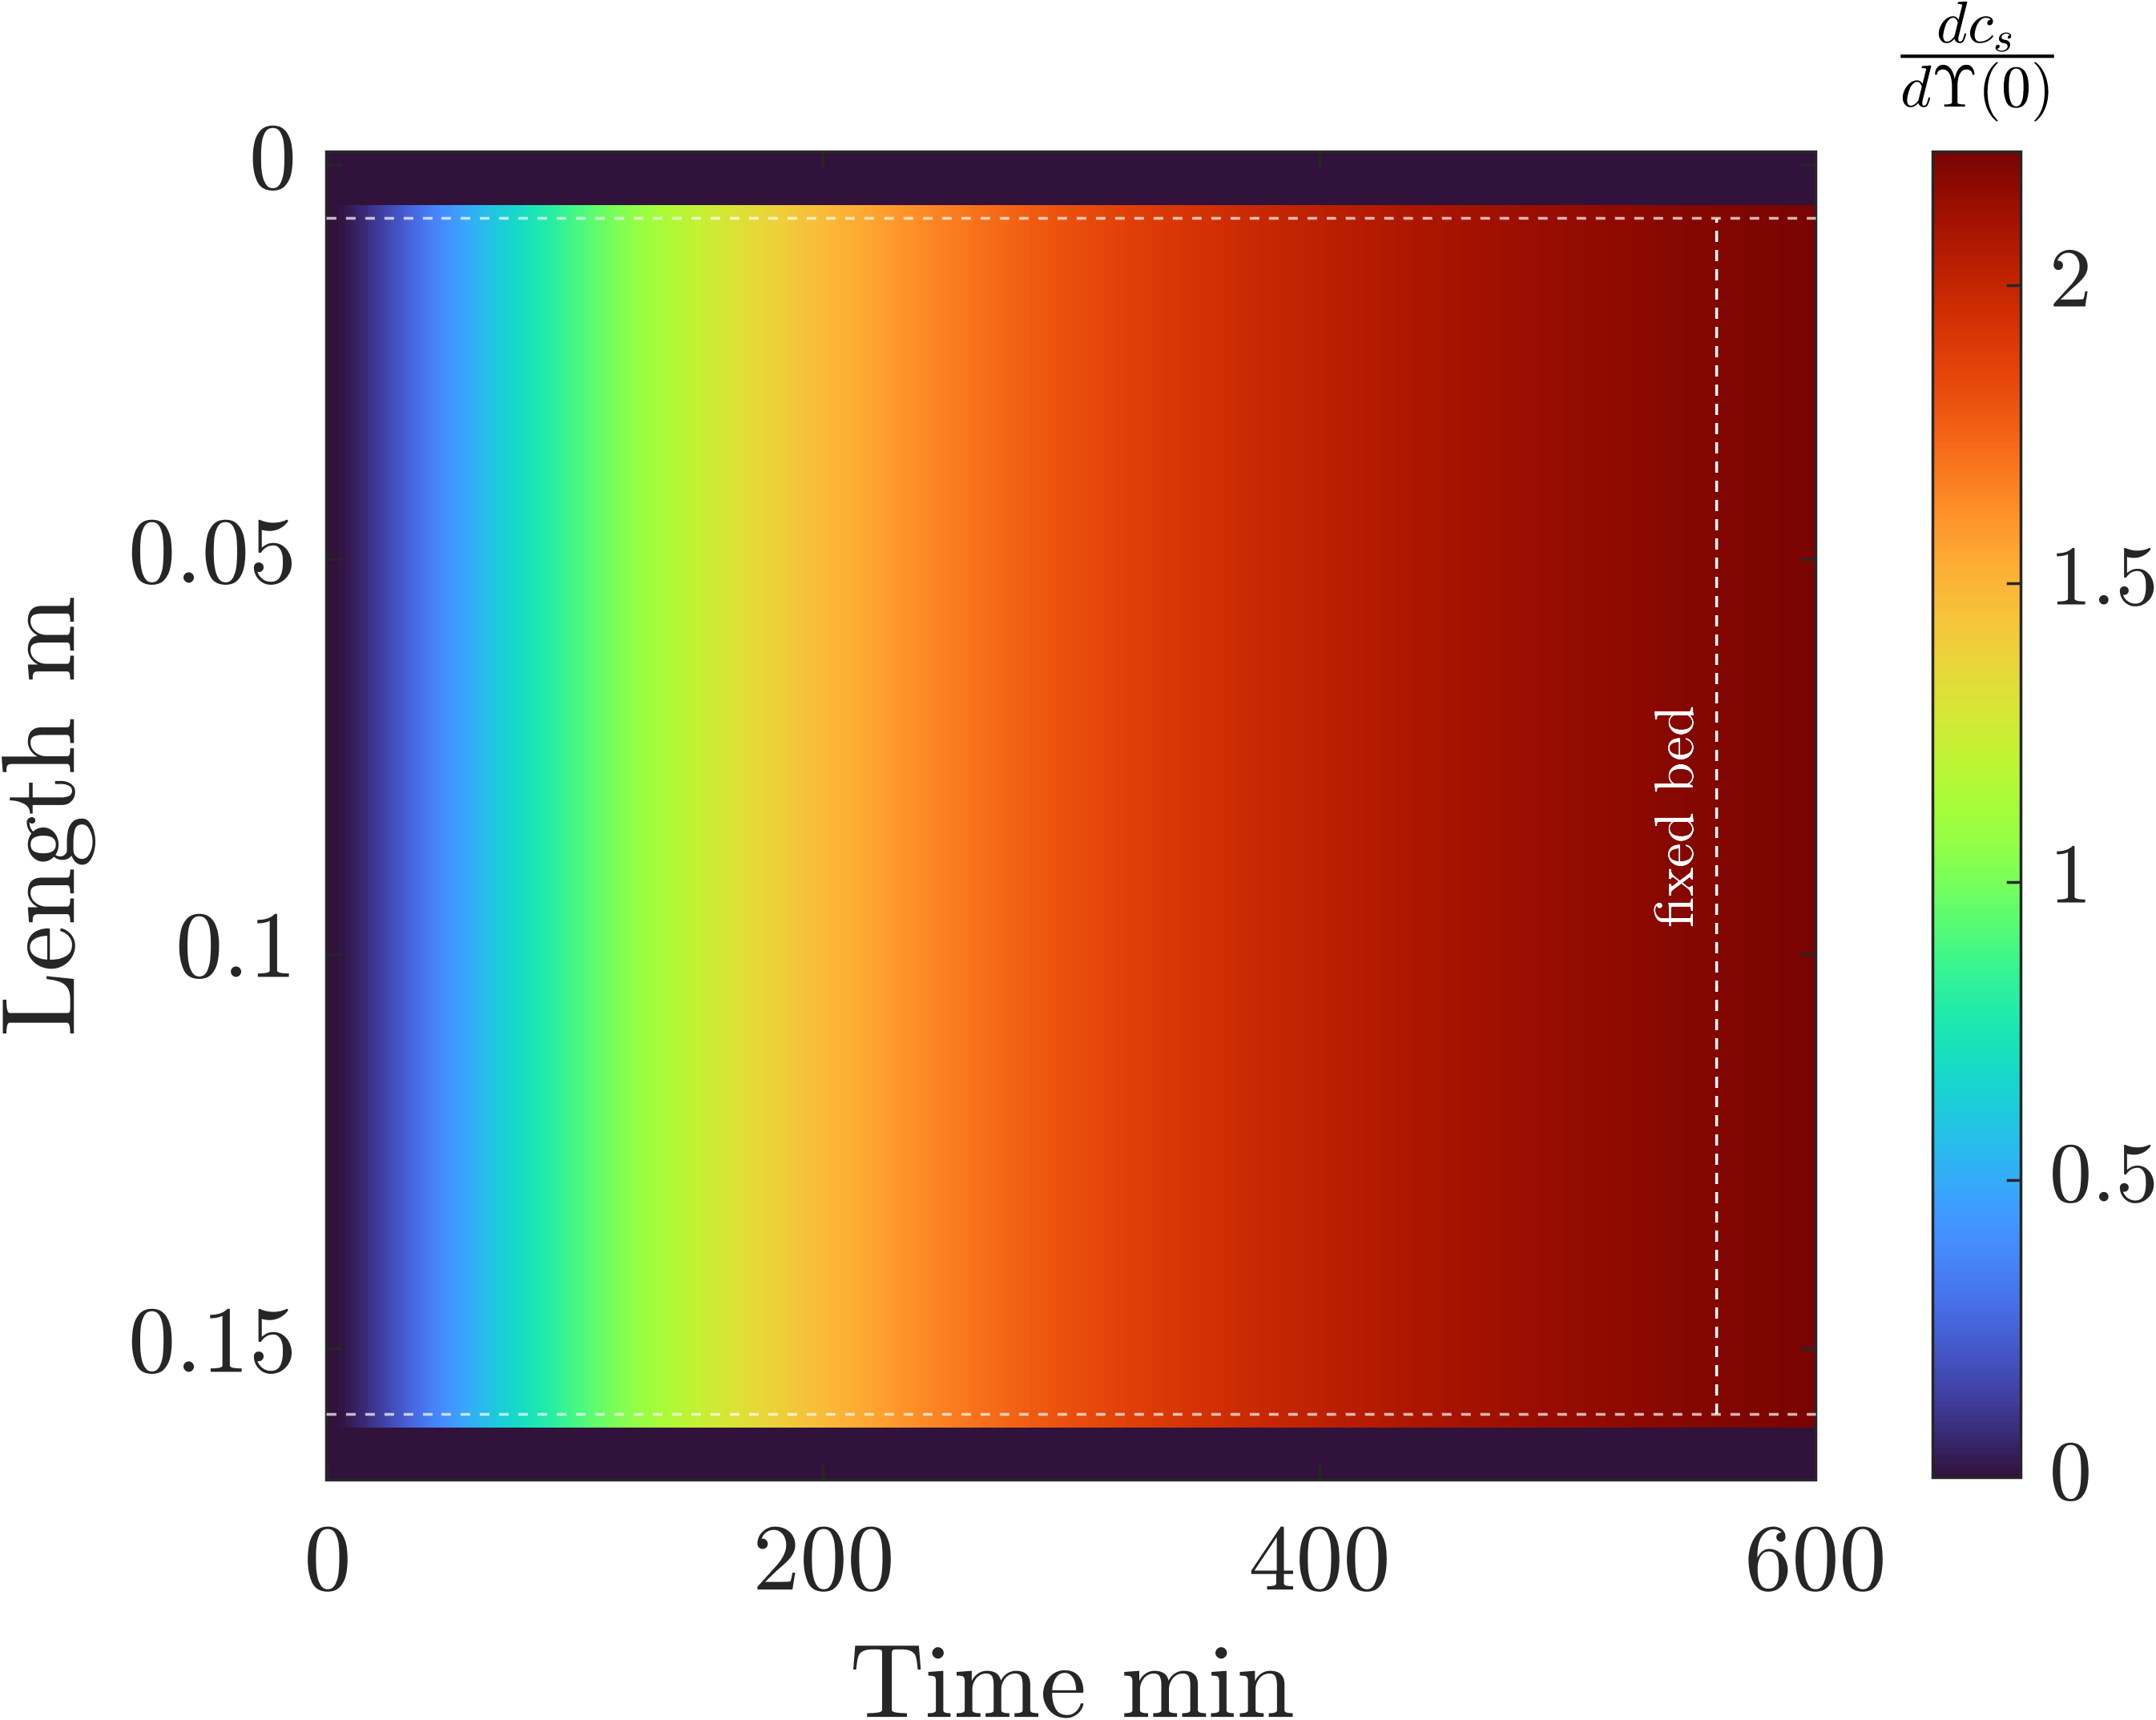
\includegraphics[trim = 0.0cm 0.0cm 0.0cm 0.0cm,clip,width=\columnwidth]{/Results_sensitivity/CS_gamma.png}
		\caption{The effect of $\Upsilon(0)$ change on $c_s$.}
		\label{fig:Sensitivty_Gamma_CS}
	\end{figure}
	
	Figure \ref{fig:Sensitivty_Gamma_CS} illustrates the sensitivity of the solute concentration in the solid phase to change into zeroth order term in the equation for $\Upsilon$. As discussed by \citet{Sliczniuk2024}, the system is far from the saturation point, which indicates that the concentration gradient is controlled mainly by $c_s$. Consequently, the extraction kinetic term acts as independent on $c_f$, which explains a uniform response in solid phase visible in Figure \ref{fig:Sensitivty_Gamma_CS}. The positive value of $\frac{dc_s}{d\Upsilon(0)}$ can be interpreted as a slower loss of the solute from particles and is observed when the extraction slows down. Because of the lower reaction rate, more solute remains in the particles initially; however, as time approaches infinity, the solute eventually diffuses out of the solid matrix. Consequently, it is expected to observ $\frac{dc_s}{d\Upsilon(0)}$ reaching a maximum and asymptotically diminish to zero.
	
	\begin{figure}[!ht]
		\centering
		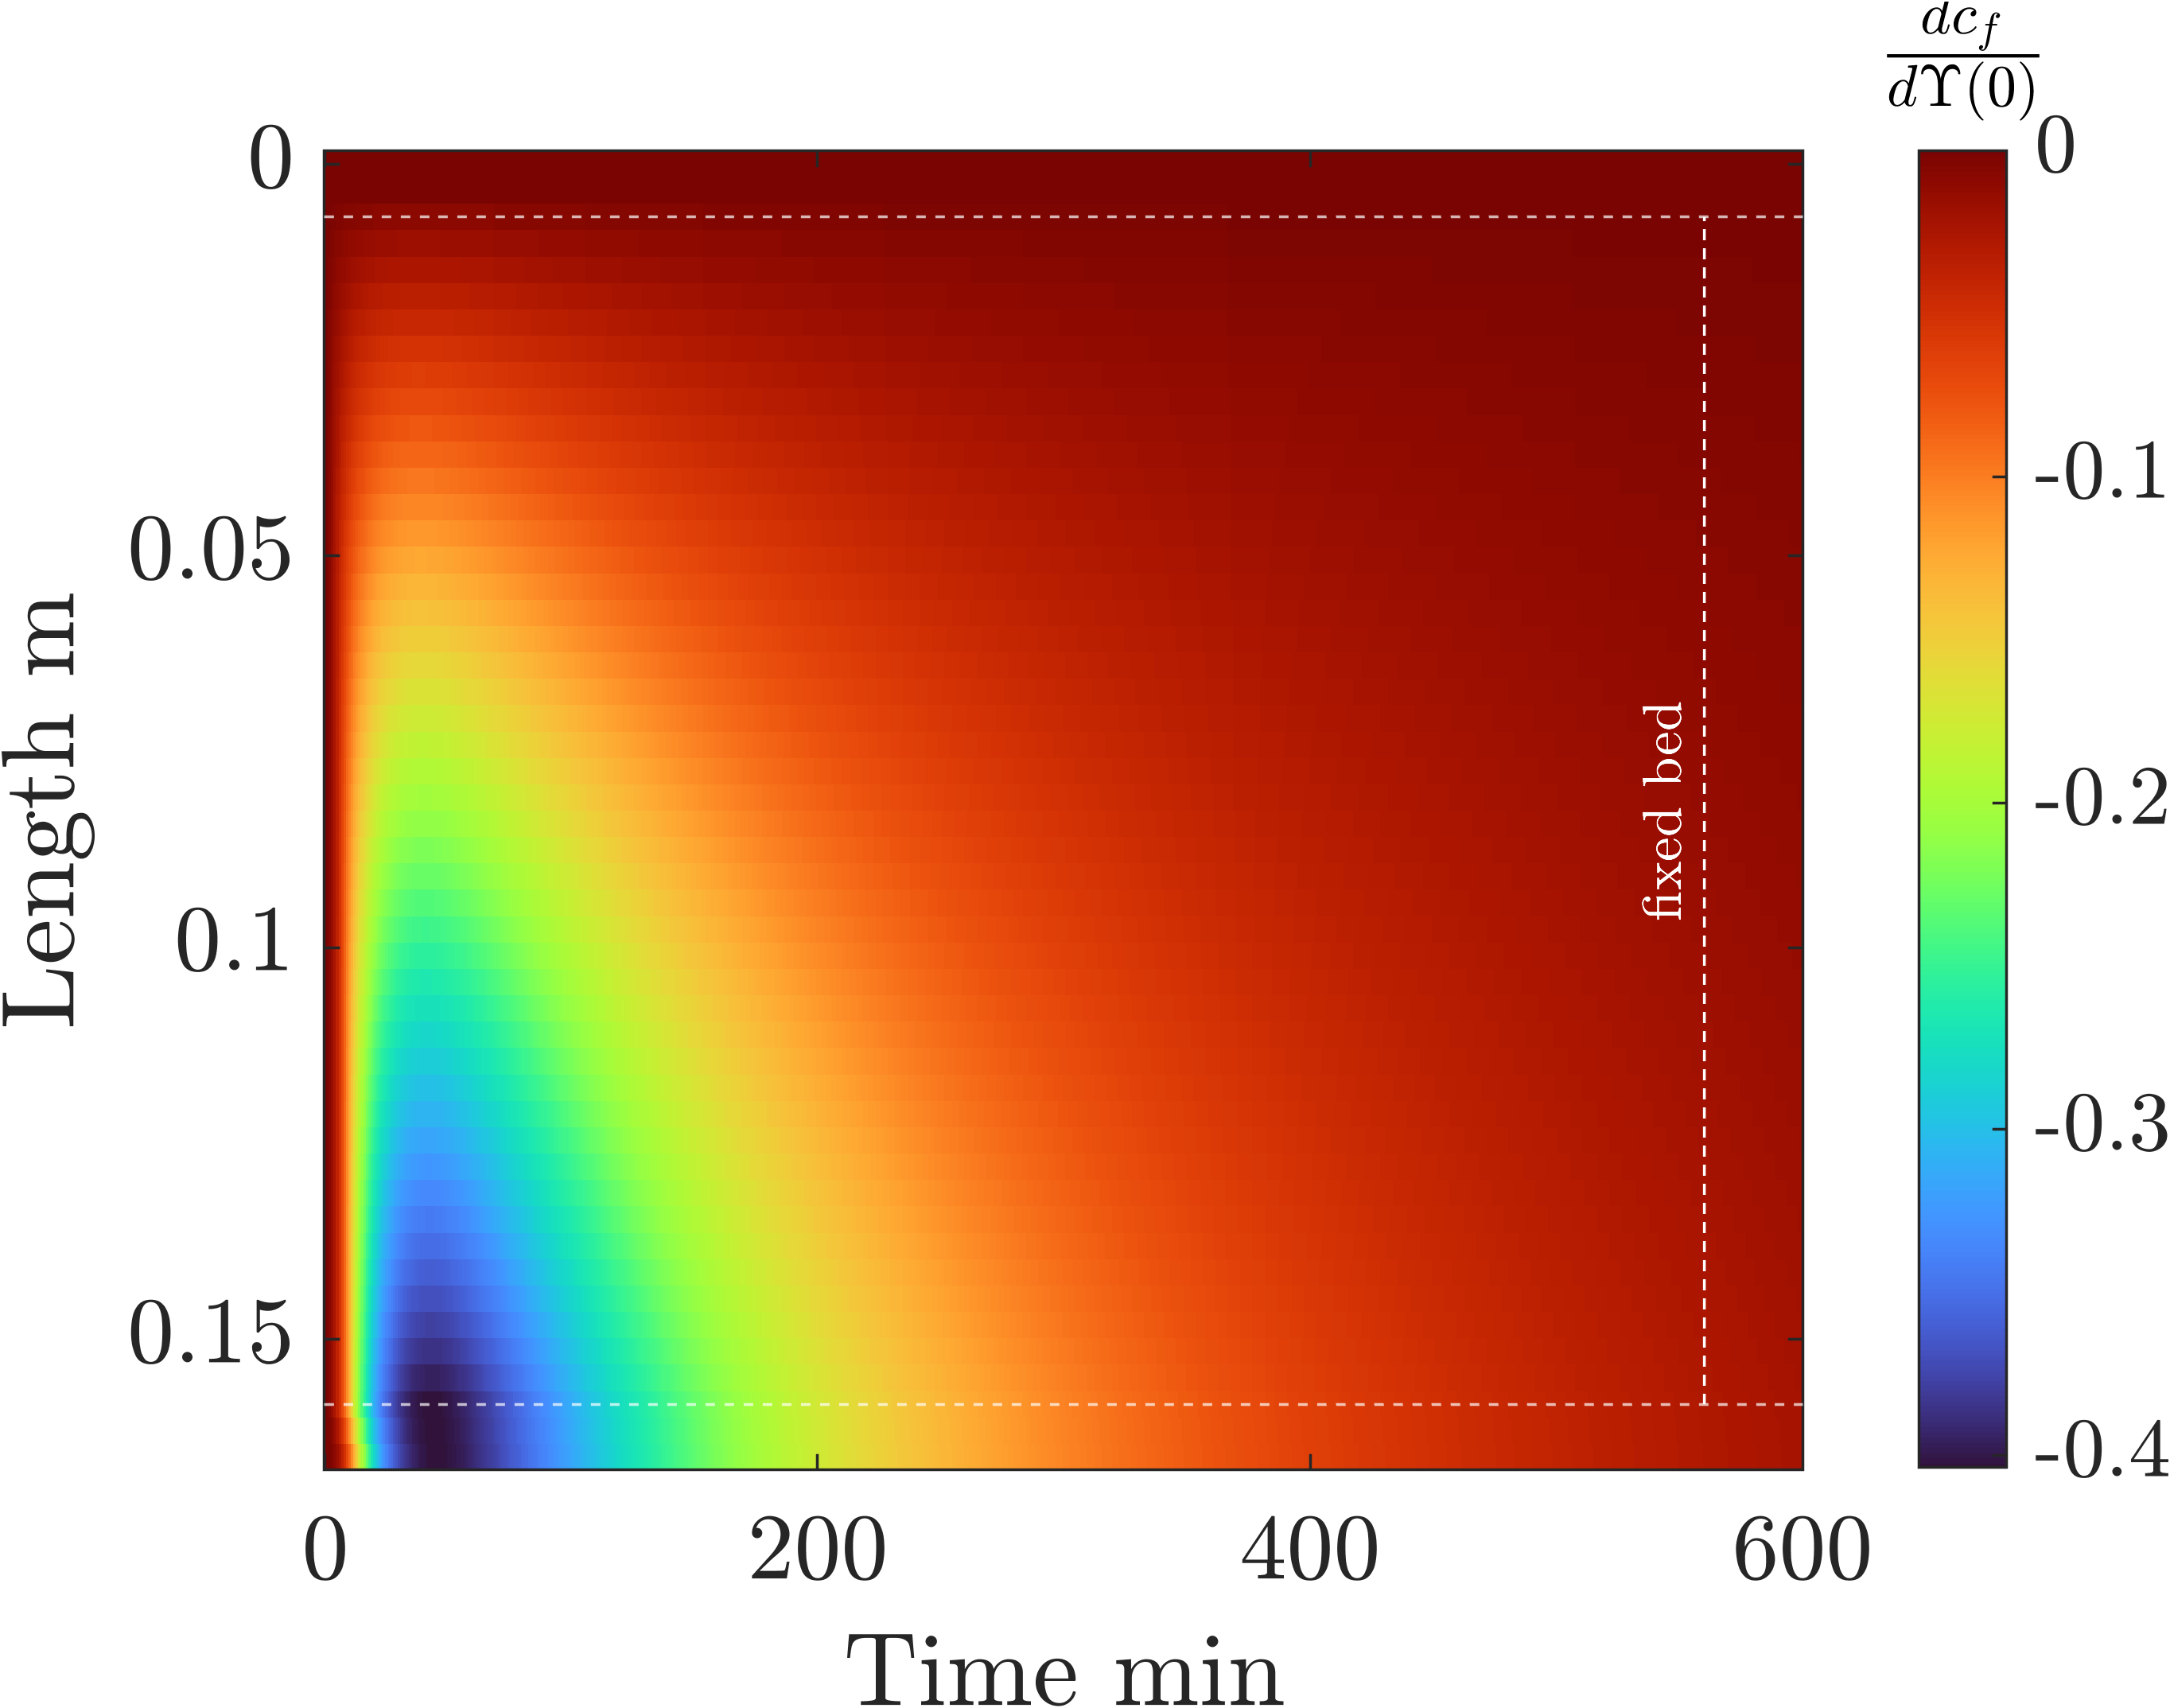
\includegraphics[trim = 0.0cm 0.0cm 0.0cm 0.0cm,clip,width=\columnwidth]{/Results_sensitivity/CF_gamma.png}
		\caption{The effect of $\Upsilon(0)$ change on $c_f$.}
		\label{fig:Sensitivty_Gamma_CF}
	\end{figure}
	
	Figure \ref{fig:Sensitivty_Gamma_CF} illustrates the sensitivity of the solute concentration in the fluid phase with respect to change into zeroth order term in the equation for $\Upsilon$. As previously discussed, the extraction rate slowed down due to increase of $\Upsilon(0)$ uniformly along the spatial domain. 
	Consequently, the solute delivered to the fluid phase decreases by an equal amount everywhere, causing a reduction in $c_f$, as indicated by the negative sign of  $\frac{dc_f}{d\Upsilon(0)}$. The spatial distribution of $\frac{dc_f}{d\Upsilon(0)}$ in the figure is non-uniform, reflecting the effects of advection. Due to mass conservation, the remaining solute reach the solid--fluid interface  more slowly, hence it is expected to observe a little positive values of $\frac{dc_f}{d\Upsilon(0)}$ in the later stage of extraction. Eventually it is expected to see sensitivities reaching zero asymptotically.
	
	\begin{figure}[!ht]
		\centering
		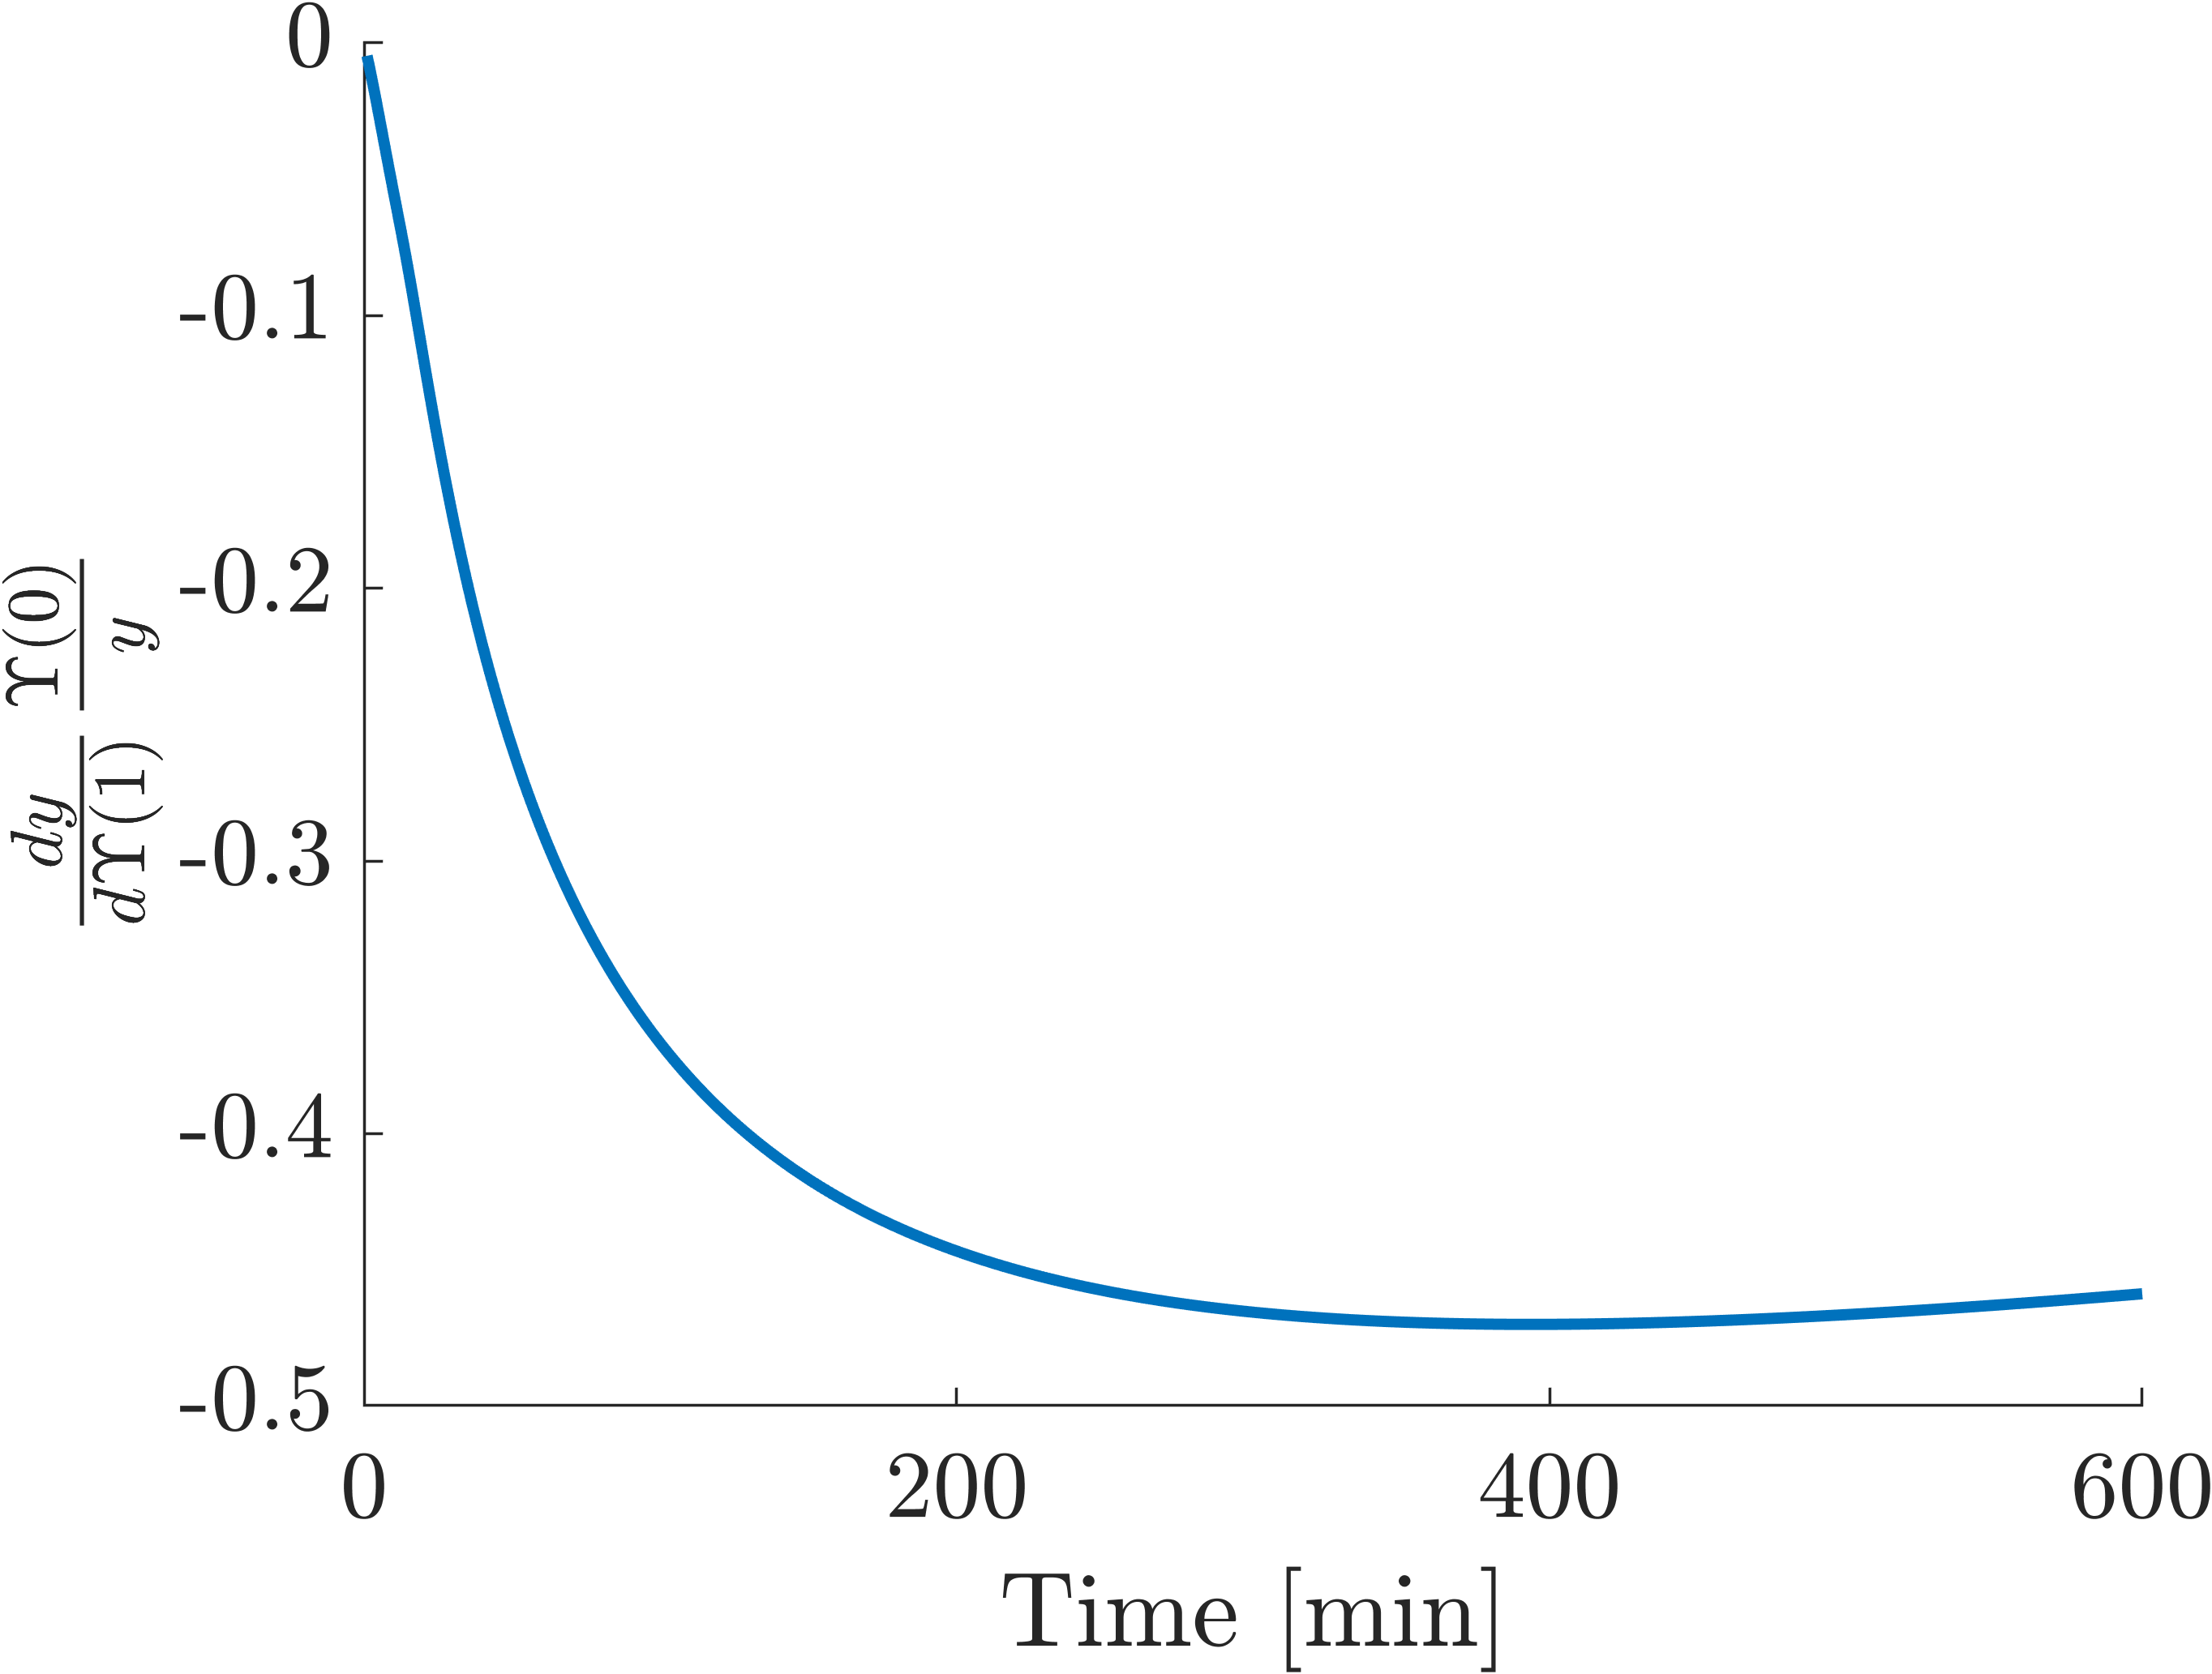
\includegraphics[trim = 0.0cm 0.0cm 0.0cm 0.0cm,clip,width=\columnwidth]{/Results_sensitivity/Y_gamma.png}
		\caption{The effect of $\Upsilon(0)$ change on $c_f$.}
		\label{fig:Sensitivty_Gamma_Y}
	\end{figure}
	
	Figure \ref{fig:Sensitivty_Gamma_Y}  shows the normalized sensitivity of the yield with respect to $\Upsilon(0)$. Due to the slower extraction rate, the sensitivity curve is characterized by negative sign. The  downward trend of the sensitivity curve can be interpreted as less solute coming out of the extractor if compared with the reference case. The curve then reaches a negative minimum (also visible in Figure \ref{fig:Sensitivty_Gamma_Y}) before the remaining solute is eventually released to the fluid phase, causing the sensitivity to approach zero asymptotically. When the sensitivity function of a dynamic system approaches zero as time goes to infinity and remains at that value, it indicates that the system's long-term behaviour becomes independent of the parameter. The parameter has only influence for the system's transient dynamics, it has no effect on the steady-state solution. This means that after the system has settled, variations in that parameter do not affect the final output. In terms of SFE, it means that all the solute has been removed from the system.
		
	\subsection{Pressure case}
	As discussed in Section \ref{CH:Governing_equations_chapter}, at low velocity, the fluid can be treated as incompressible, which results in the instant propagation of pressure throughout the system, enabling a single pressure value to be considered for the entire system. In response to a pressure change, the energy equation experiences a simultaneous deviation across the entire spatial domain. This pressure change impacts the fluid temperature within the computational domain, while boundary values are constrained by conditions specified at the domain's extremes. Dirichlet boundary conditions impose a fixed temperature value at the inlet, creating a thermal gradient that propagates through the system. Alternatively,  Neumann boundary conditions specify a heat flux at the extremes. The zero Neumann boundary conditions are applied to ensure a uniform response to the pressure change of temperatures at the inlet, outlet, and within the extractor.
		
	\begin{figure}[!ht]
		\centering
		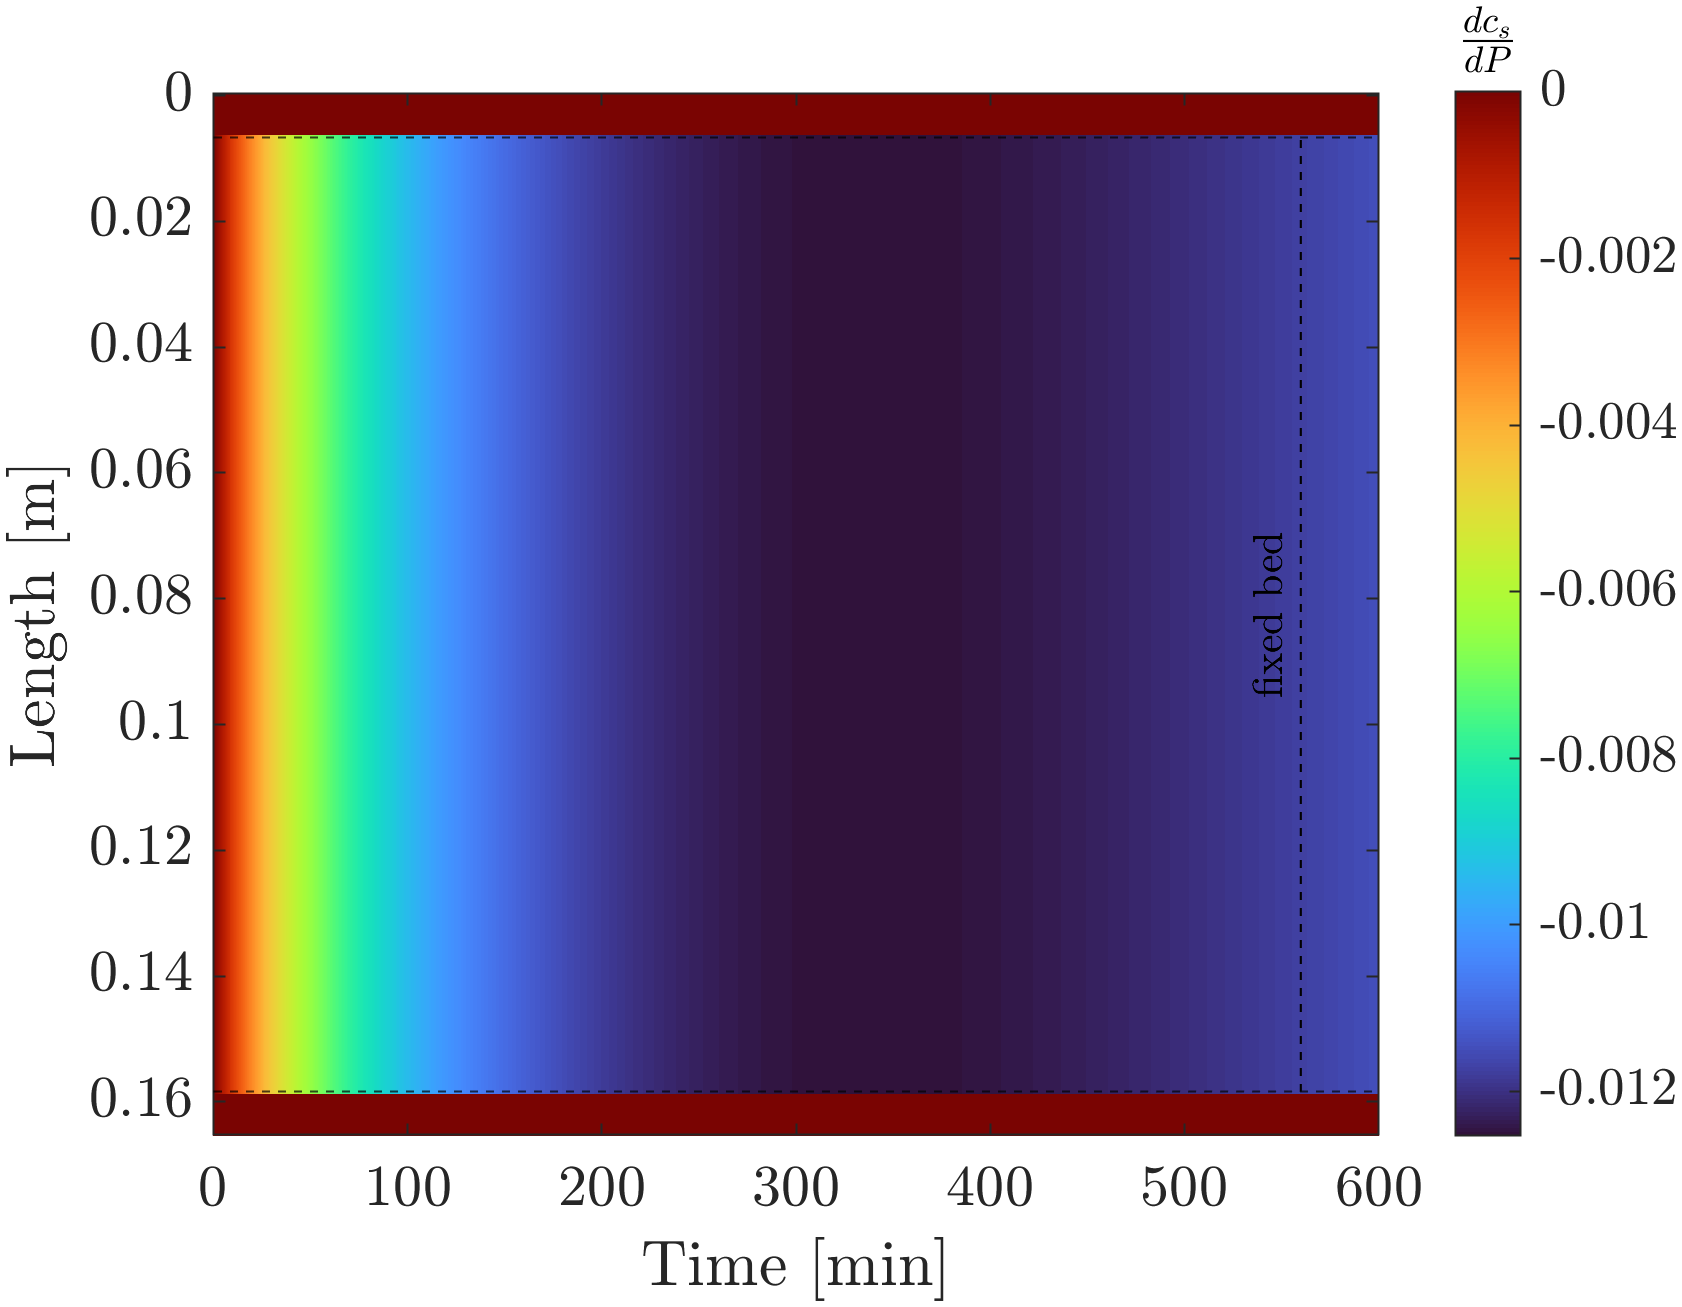
\includegraphics[trim = 0.0cm 0.0cm 0.0cm 0.0cm,clip,width=\columnwidth]{/Results_sensitivity/CS_P.png}
		\caption{The effect of $P_{in}$ change on $c_s$.}
		\label{fig:Sensitivty_P_CS}
	\end{figure}
	
	Figure \ref{fig:Sensitivty_P_CS} illustrates the sensitivity of the solute concentration in the solid phase to pressure changes. As discussed in Section \ref{CH: Continuity}, the velocity of a fluid is inversely proportional to its density, indicating that increased pressure reduces the fluid velocity. This results in an extended residence time, allowing for longer interaction between the solute and solvent. Initially, the extraction process operates in the kinetic-controlled regime, where the concentration gradient is high, and solute solubility is the limiting factor. As noted by \citet{Sliczniuk2024}, the system is considered far from saturation, which explains the low initial system response. This low initial response was also observed in the sensitivity analysis by \citet{Fiori_2007}. The system's response becomes more pronounced as the concentration gradient decreases and the extraction shifts from the kinetic-controlled to the diffusion-controlled regime. In Figure \ref{fig:Sensitivty_P_CS}, all $\frac{dc_s}{dP}$ values are negative, which indicates a faster mass transfer from the solid phase, corresponding to enhanced mass transfer.  Over time, as the amount of solute decreases, it becomes a limiting factor, reducing the effect of pressure changes on the system. Eventually, the sensitivities approach zero asymptotically as the solute is washed out of the bed.
	
	\begin{figure}[!ht]
		\centering
		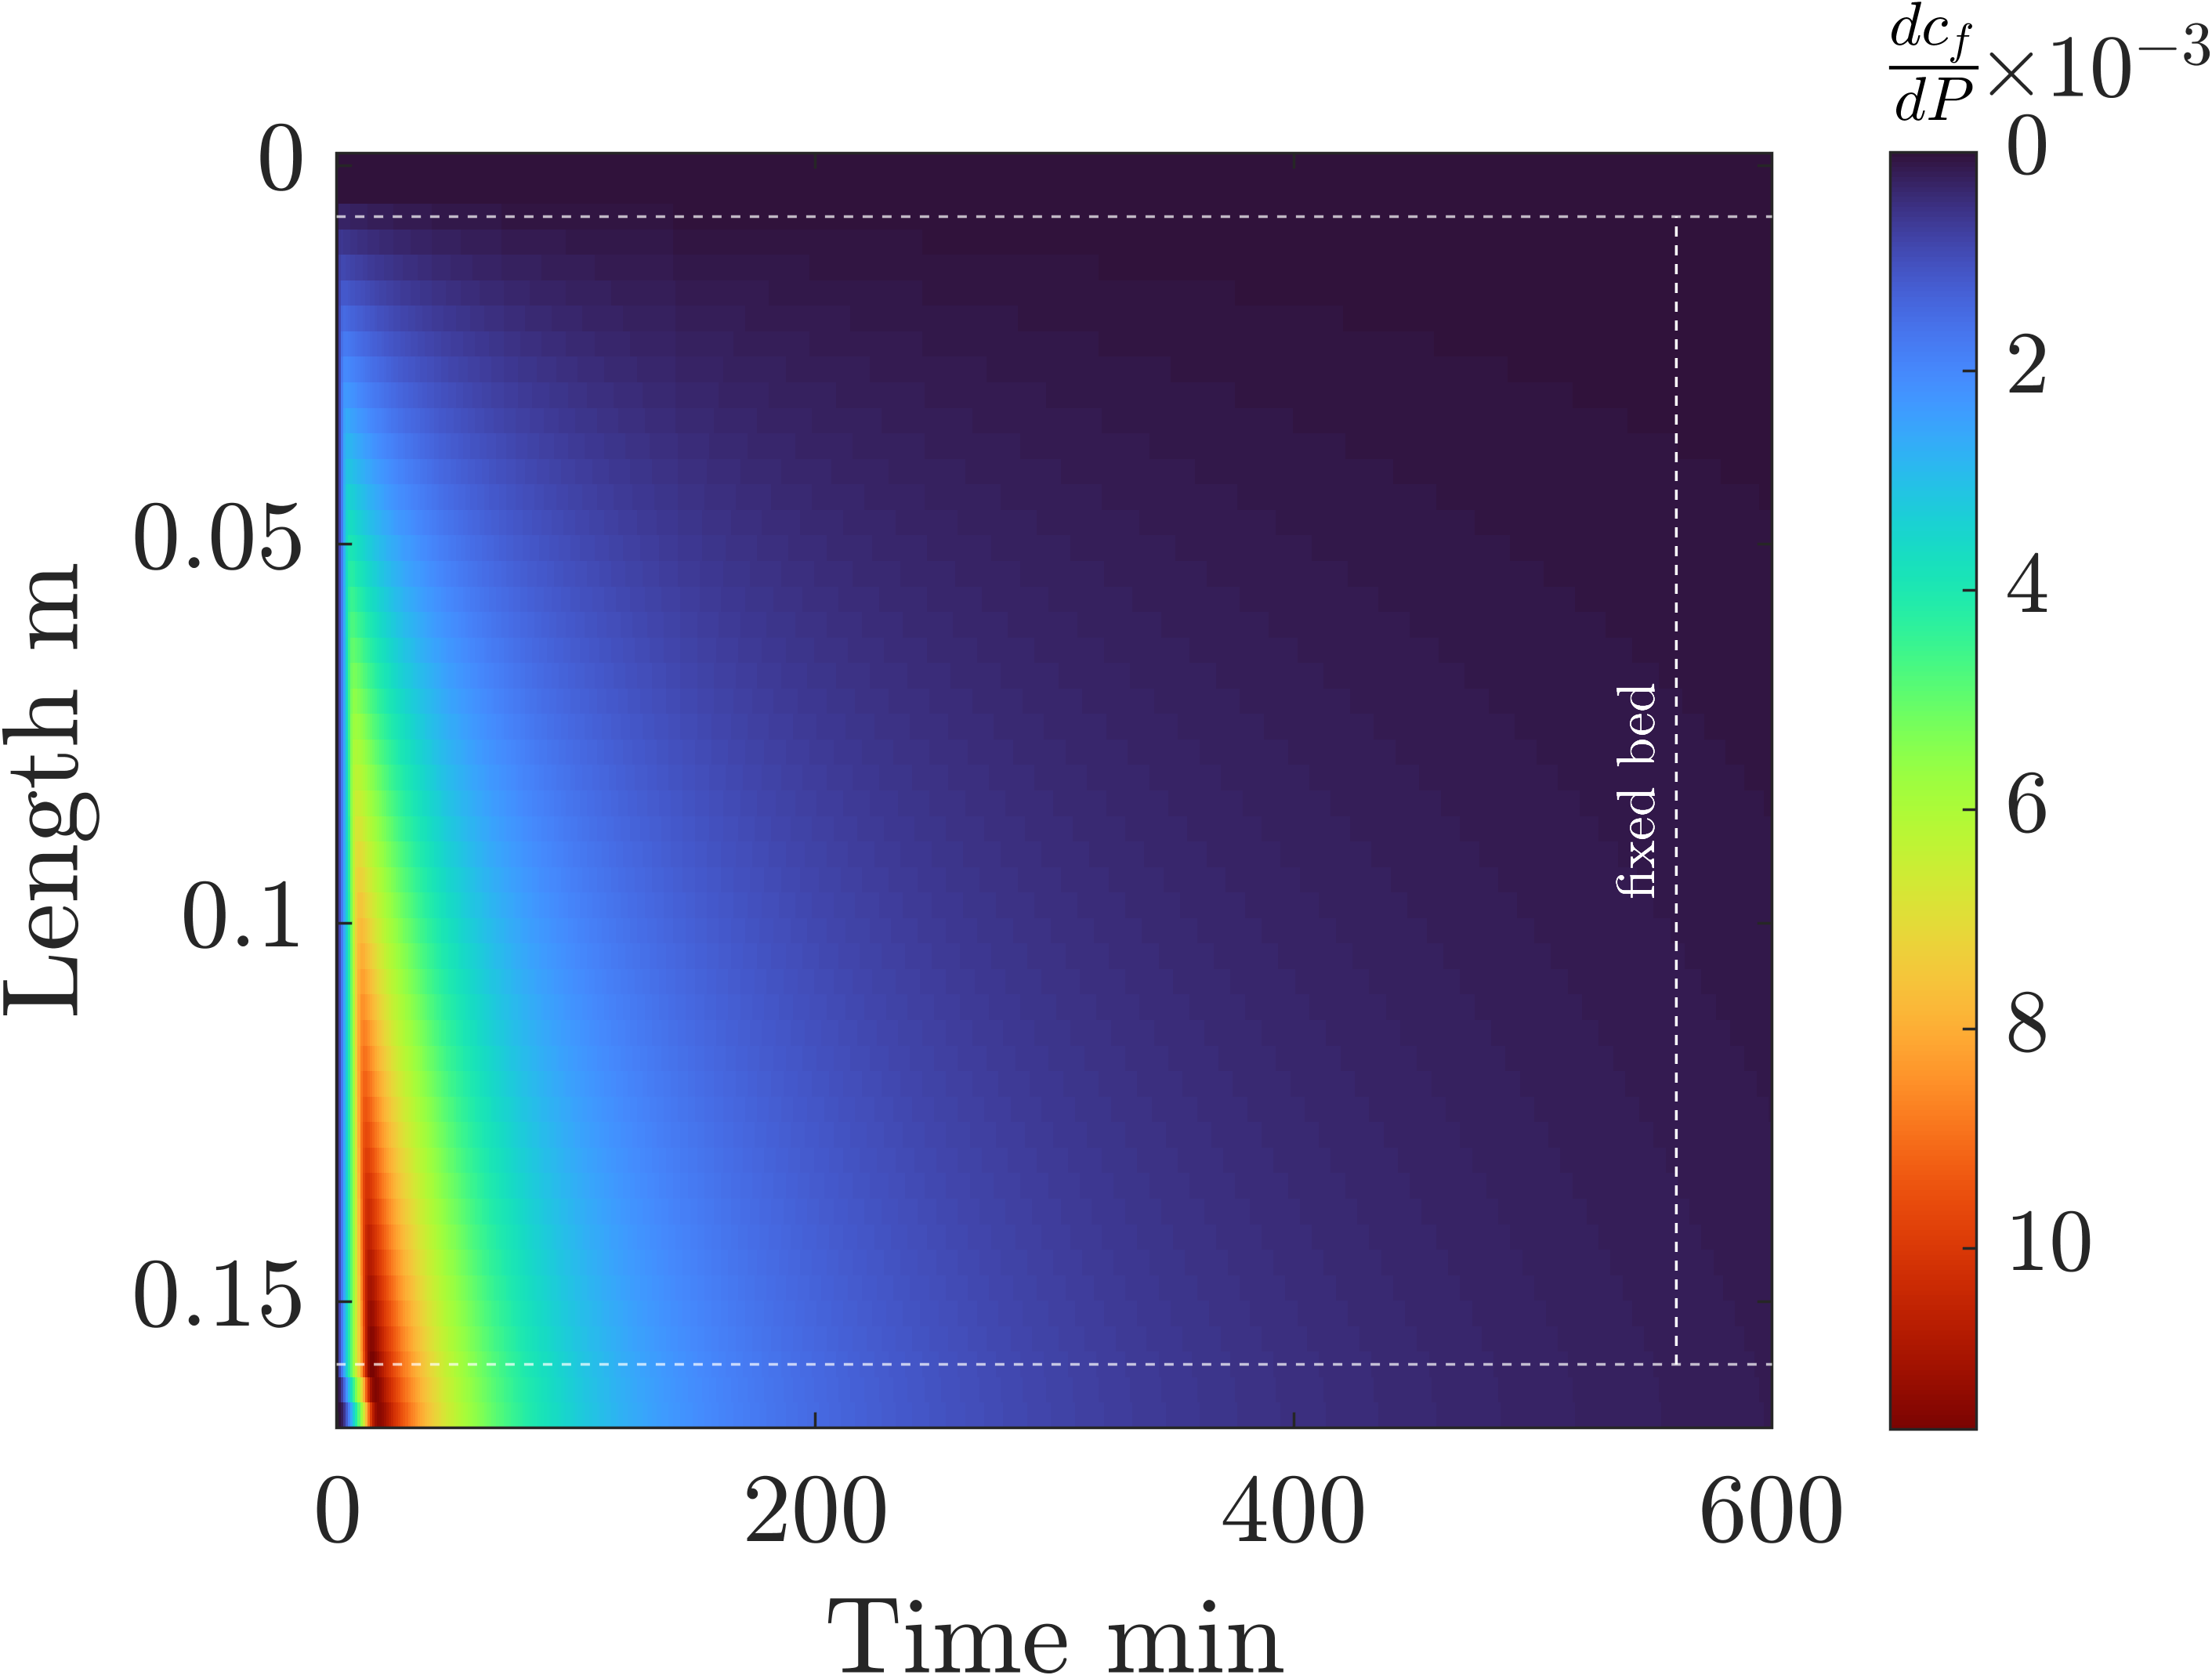
\includegraphics[trim = 0.0cm 0.0cm 0.0cm 0.0cm,clip,width=\columnwidth]{/Results_sensitivity/CF_P.png}
		\caption{The effect of $P_{in}$ change on $c_f$.}
		\label{fig:Sensitivty_P_CF}
	\end{figure}
	
	
	Figure \ref{fig:Sensitivty_P_CF} illustrates the sensitivity of solute concentration in the fluid phase to pressure changes. Compared to Figure \ref{fig:Sensitivty_P_CS}, the dynamic behaviour of fluid phase sensitivities is more apparent. Due to advection, the sensitivities related to the fluid phase move across the system in the direction of flow. Initially, the system response is low despite the pressure increase improving mass transfer, reflecting the previously discussed idle period. As the process continues, the sensitivities increase, indicating faster mass transfer from the solid phase. The corresponding improvement in the mass transfer from the solid particles to the fluid is represented by the positive values in Figure \ref{fig:Sensitivty_P_CF}. When the solute in the solid phase becomes a limiting factor, the extraction rate slows, and sensitivities eventually approach zero asymptotically.
	
	Figure \ref{fig:Sensitivty_P_y} shows how sensitive the extraction yield is to pressure changes over an extended period for various pressure values. Initially, all sensitivity curves remain nearly flat, indicating a delayed response in the system. Due to the reduced fluid velocity, the solute reaches the extractor's outlet later, causing minor negative sensitivities to appear. Once the solute exits the extractor, the sensitivity curves rise. Positive yield sensitivities indicate improved process efficiency and enhanced mass transfer. The peak in $\frac{dy}{dP_{in}}$ represents the point of greatest deviation from the original system. Eventually, the sensitivities decline and converge towards zero as the concentration gradient becomes a limiting factor, reducing the impact of enhanced mass transfer.
	
	\begin{figure}[!ht]
		\centering
		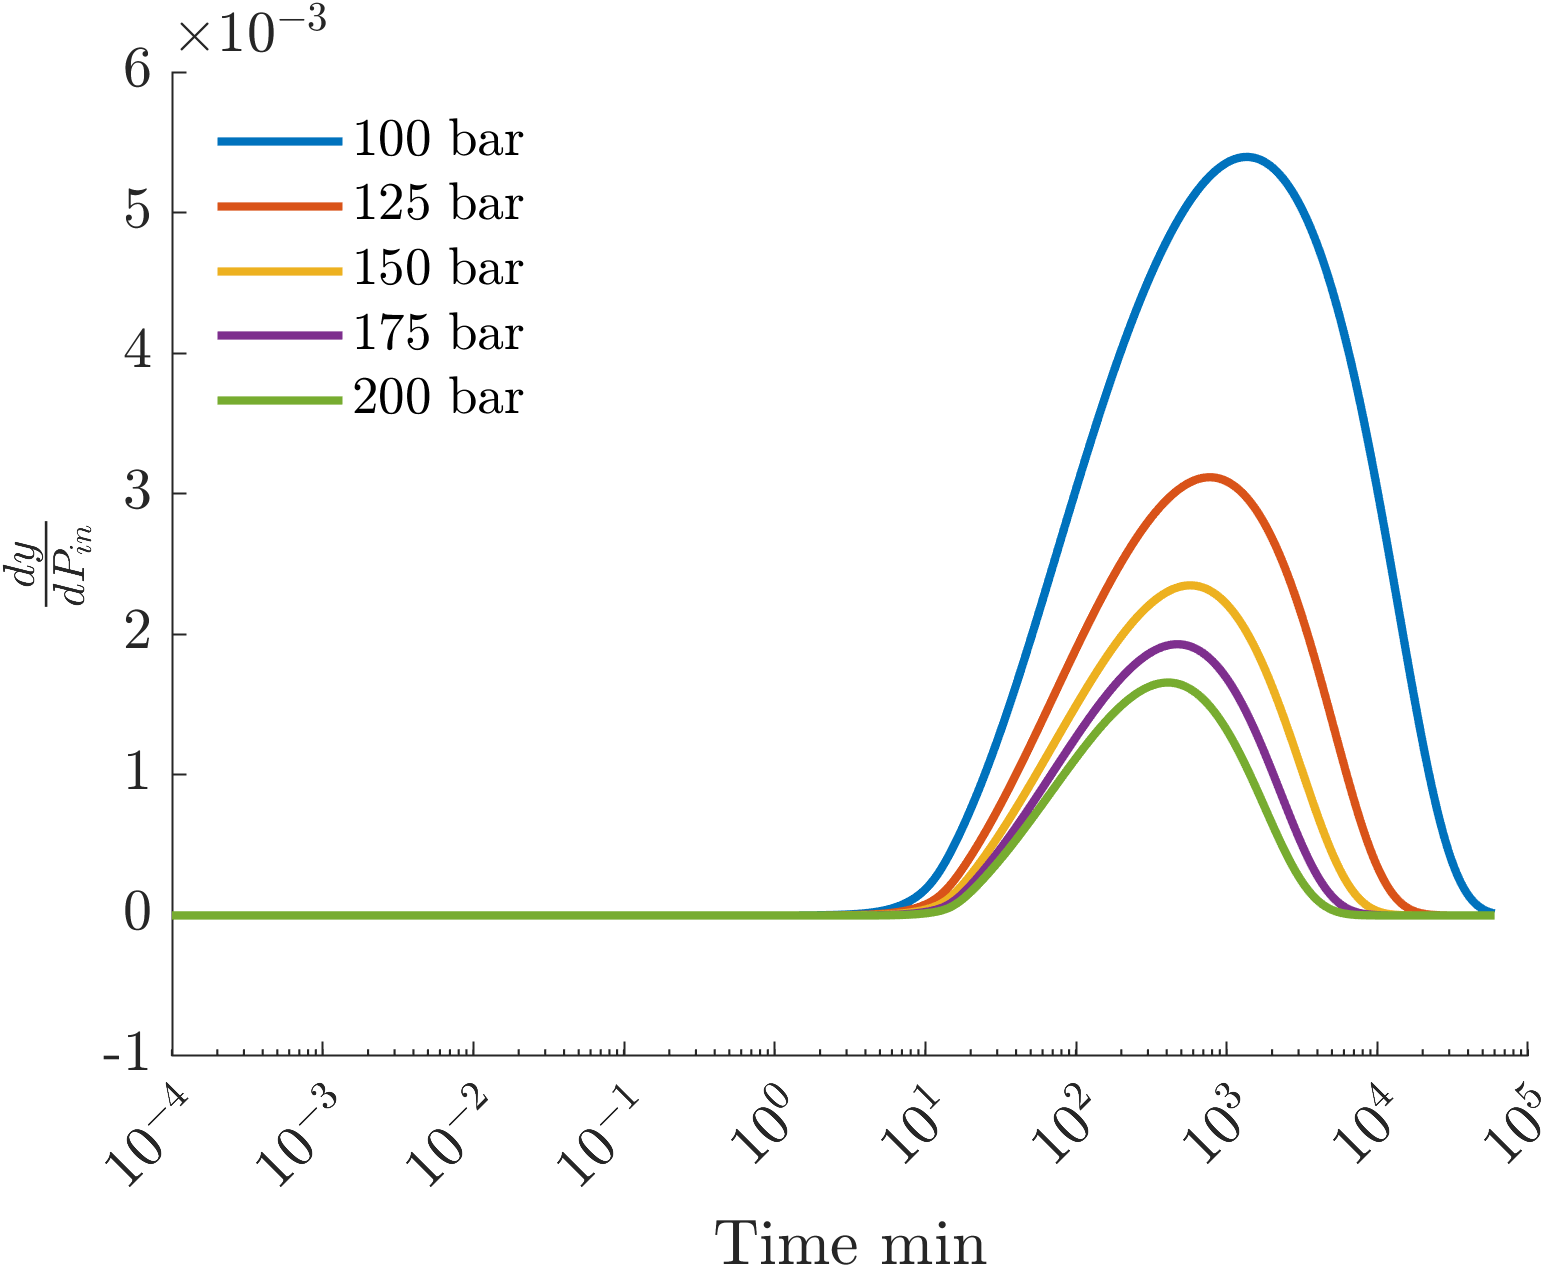
\includegraphics[trim = 0.0cm 0.0cm 0.0cm 0.0cm,clip,width=\columnwidth]{/Results_sensitivity/Yield.png}
		\caption{The effect of $P_{in}$ change on $y(t)$.}
		\label{fig:Sensitivty_P_y}
	\end{figure}
	
	As presented in Figure \ref{fig:Sensitivty_P_y}, higher sensitivities are observed for a low-pressure system. At lower pressures, the supercritical fluid has lower density and solvating power, which results in less efficient extraction, as shown by data given by \citet{Sliczniuk2024}. Small changes in pressure at low pressures can significantly impact the solute's solubility and, consequently, the extraction yield. Moreover, near the critical point, small changes in pressure can lead to significant changes in the physical properties of the supercritical fluid, such as density and viscosity, and therefore to higher sensitivity of the system state-space.
	
	\begin{figure}[!hb]
		\centering
		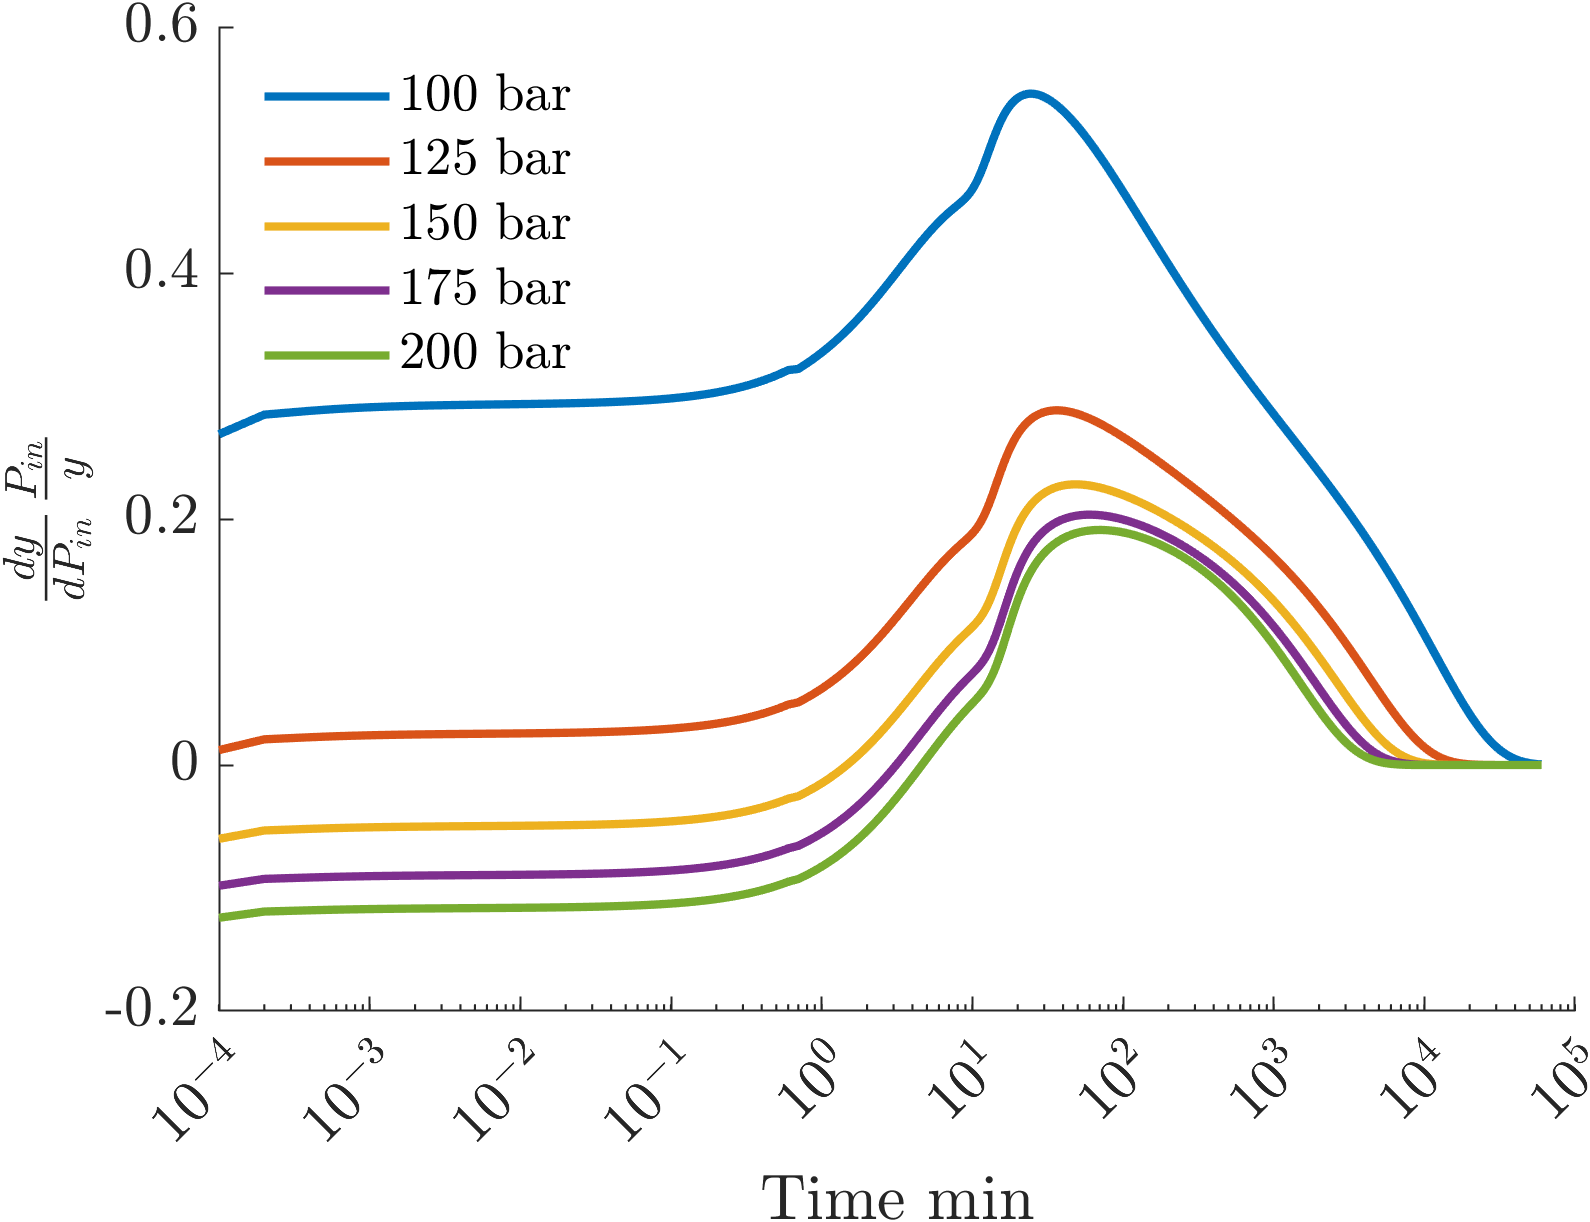
\includegraphics[trim = 0.0cm 0.0cm 0.0cm 0.0cm,clip,width=\columnwidth]{/Results_sensitivity/Yield_Multiple_normalized.png}
		\caption{The effect of $P_{in}$ change on $y(t)$ after normalization.}
		\label{fig:Sensitivty_P_y_norm}
	\end{figure}
			
	Figure \ref{fig:Sensitivty_P_y_norm} illustrates the time evolution of the normalized sensitivity coefficients of the extraction yield. Unlike the raw sensitivities shown in Figure \ref{fig:Sensitivty_P_y}, the normalized sensitivities do not start from zero. This is due to the absence of the exact initial time point on the logarithmic time axis. The pressure change impacts the system instantaneously and uniformly, leading to a rapid initial change in the normalized sensitivities. This behaviour is analogous to a step change, where the system's response to the perturbation is immediate. Initially, the sensitivity curves remain flat. The increase in normalized sensitivity begins when the solute reaches the system's outlet and becomes detectable. After reaching their respective maxima, the sensitivity curves decrease as the concentration gradient driving the extraction diminishes over time. Ultimately, all curves approach zero, reflecting that all the solute was removed from the solid phase.
	
	While this interpretation of normalized sensitivities is straightforward, it is important to note that extrapolating for large parameter changes can lead to inaccurate results. In dynamic systems, local sensitivity analysis quantifies how the system state or output varies over time in response to small parameter perturbations. If the perturbation is large, the derivative-based definition of sensitivity (or sensitivity equations) becomes invalid unless the system is linear. Consequently, the conclusions from local sensitivity analysis cannot be reliably scaled to large parameter changes. This limitation makes reproducing of sensitivity results in laboratory conditions challenging, given the finite precision of experimental equipment.
	
	\section{Conclusions} \label{CH: Conclusion}
	
	Sensitivity analysis is a tool used to understand how the parameters of the model affect its output. The presented formulation involves derivative-based local sensitivity analysis of the model solution with respect to selected parameters and controls. This work implemented automatic differentiation to derive the sensitivity equations. The results of the local sensitivity analysis are model specific and consider only a small region of parameter space, so the conclusions derived from such an analysis are limited to local conditions. Although local sensitivity analysis can be performed with respect to any model parameter, this study focuses on the selected parameters of the empirical correlation and operating conditions.
	
	The motivation for performing a sensitivity analysis is to validate the model, evaluate how parameter variations affect its outputs, and identify potential modelling errors or unfeasible behaviours. This work assessed the influence of the selected parameter from the empirical correlation for $\Upsilon$. The analysis showed that increment of $\Upsilon(0)$ slows down the extraction rate, leading to negative values of $\frac{dc_s}{d\Upsilon(0)}$ and $\frac{dy}{d\Upsilon(0)}$, and alternating values of $\frac{dc_f}{d\Upsilon(0)}$. These findings align with the physical interpretation of $\Upsilon(0)$. The effect of the parameter change can be summarised by extreme and final values of the normalised sensitivity of the output (0.47 and 0, respectively).
	
	The second analysis was to examine influence of operating conditions on the SFE model, particularly the pressure effect. Given that the results of the local sensitivity analysis depend on the operating point, the analysis was conducted at different pressures. For all the investigated operating conditions, it was observed that the pressure increment enhanced mass transfer, leading to a faster mass transfer of solute from the particles. Consequently, negative sensitivities can be observed in sensitivity diagrams for the solid phase. The corresponding response in the fluid phase is characterized by positive-valued sensitivities, indicating that higher quantity of solute is transported into the fluid phase. As a result, the extraction yield is improved and characterized by positive sensitivities. To compare the influence of various pressures, normalized sensitivity coefficients were used, showing values between -$0.17$ and $0.6$. The overall effect of each parameter was assessed by integrating the yield sensitivity curves over extended simulation time (until all sensitivities approached zero). Table \ref{table:Cumulative_integral} presents initial, maximum, and cumulative values of the integral of the normalized sensitivity coefficients. The cumulative integrals' positive sign confirms that increasing pressure improves the extraction yield under all investigated conditions. The relative magnitudes of these integrals can be used to identify the operating conditions where pressure variations are the most influential. Table \ref{table:Cumulative_integral} also shows that the system response change depending on the physical properties of CO$_2$ and the flow regime. 
	
	\begin{table}[h!]
		\adjustbox{max width=\columnwidth}{%
		\centering
		\begin{tabular}{|l| c c c c c|} 
			\hline
			Pressure case & 100 & 125 & 150 & 175 & 200 \\ 
			\hline
			Initial normalized sensitivity & 0.25 & -0.08 & -0.13 & -0.15 & -0.17 \\ 
			Max normalized sensitivity & 0.52 & 0.28 & 0.18 & 0.15 & 0.13 \\ 
			Cumulative integral & 31487 & 8548 & 4462 & 2825 & 1939 \\ 
			\hline
		\end{tabular} }
		\caption{Values of the cumulative integral of the yield sensitivity.}
		\label{table:Cumulative_integral}
	\end{table}
	
	The findings of this work are particularly valuable for industrial-scale supercritical extraction processes, where achieving both operational efficiency and product quality can be challenging. The local sensitivity analysis demonstrates that even small adjustments in operating parameters can yield disproportionately large effects on extraction rates, especially near the fluid’s critical point. By quantifying how parameter variations affect the model states, the high-efficiency operating setpoints can be identified. Moreover, linking local sensitivity analysis to numerical optimization establishes a systematic framework for industrial process design and scale-up. Rather than relying heavily on trial-and-error or resource-intensive pilot studies, the model-based approach can be used to pre-identify the region of interests. This approach reduces both the time and material costs needed to reach profitable extraction rates, moving industrial operations toward cost-effective production.
	
	\section*{Acknowledgements} 
	This work was supported by: NovelBaltic, CEForestry (IBC), BIO4P (BF).
	
	% ===================================================
	% Bibliography
	% ===================================================
	%% Loading bibliography style file
	\clearpage
	%\newpage
	%\bibliographystyle{model1-num-names}
	\bibliographystyle{unsrtnat}
	\bibliography{mybibfile}
	
	%\clearpage
	
	\nomenclature[A]{\(P\)}{pressure \nomunit{bar}}
	\nomenclature[A]{\(T\)}{temperature \nomunit{K}}
	\nomenclature[A]{\(T_{in}\)}{inlet temperature \nomunit{K}}
	\nomenclature[A]{\(T_{out}\)}{outlet temperature \nomunit{K}}
	\nomenclature[A]{\(F\)}{mass flow rate \nomunit{kg/s}}
	\nomenclature[A]{\(u\)}{superficial velocity \nomunit{m/s}}
	\nomenclature[A]{\(v\)}{linear velocity \nomunit{m/s}}
	\nomenclature[A]{\(z\)}{spatial direction \nomunit{m}}
	\nomenclature[A]{\(e\)}{internal energy \nomunit{J/kg}}
	\nomenclature[A]{\(h\)}{enthalpy \nomunit{J}}
	\nomenclature[A]{\(t\)}{time \nomunit{s}}
	\nomenclature[A]{\(t_f\)}{total extraction time \nomunit{s}}
	\nomenclature[A]{\(t_0\)}{initial extraction time \nomunit{s}}
	\nomenclature[A]{\(A\)}{total cross-section of the bed \nomunit{m$^2$}}
	\nomenclature[A]{\(A_f\)}{cross-section of the bed occupied by the fluid \nomunit{m$^2$}}
	\nomenclature[A]{\(c_f\)}{concentration of solute in the fluid phase \nomunit{kg/m$^3$}}
	\nomenclature[A]{\(c_{f0}\)}{initial concentration of solute in the fluid phase \nomunit{kg/m$^3$}}
	\nomenclature[A]{\(c_f^*\)}{concentration of solute at the solid-fluid interface \nomunit{kg/m$^3$}}
	\nomenclature[A]{\(c_s\)}{concentration of solute in the solid phase \nomunit{kg/m$^3$}}
	\nomenclature[A]{\(c_{s0}\)}{initial concentration of solute in the solid phase \nomunit{kg/m$^3$}}
	\nomenclature[A]{\(c_s^*\)}{concentration of solute at the solid-fluid interface \nomunit{kg$^3$}}
	\nomenclature[A]{\(c_p\)}{concentration of solute in the core of a pore \nomunit{kg/m$^3$}}
	\nomenclature[A]{\(c_{pf}\)}{concentration of solute at the pore opening \nomunit{kg/m$^3$}}
	\nomenclature[A]{\(D_e^M\)}{axial diffusion coefficient \nomunit{m$^2$/s}}
	\nomenclature[A]{\(r_e\)}{mass transfer kinetic term \nomunit{kg/m$^3$/s}}
	\nomenclature[A]{\(L\)}{length of the fixed bed \nomunit{m}}
	\nomenclature[A]{\(S\)}{sensitivity equations}
	\nomenclature[A]{\(\textbf{G}\)}{augmented system}
	\nomenclature[A]{\(\dot{S}\)}{time derivative of the sensitivity equations}
	\nomenclature[A]{\(\bar{S}\)}{sensitivity matrix}
	\nomenclature[A]{\(\bar{J}_x\)}{Jacobian matrix with respect to the state variables}
	\nomenclature[A]{\(\bar{J}_\Theta\)}{Jacobian matrix with respect to the parameters}
	%\nomenclature[A]{\(\mathcal{L}\)}{Log-likelihood function}
	\nomenclature[A]{\(l\)}{characteristic dimension of particles \nomunit{m}}
	\nomenclature[A]{\(D_i\)}{internal diffusion coefficient \nomunit{m$^2$/s}}
	\nomenclature[A]{\(D_i^R\)}{reference value of internal diffusion coefficient \nomunit{m$^2$/s}}
	\nomenclature[A]{\(r\)}{particle radius \nomunit{m}}
	\nomenclature[A]{\(k_p\)}{volumetric partition coefficient \nomunit{-}}
	\nomenclature[A]{\(k_m\)}{mass partition coefficient \nomunit{-}}
	\nomenclature[A]{\(y\)}{extraction yield \nomunit{g}}
	%\nomenclature[A]{\(Y\)}{Yield measurement \nomunit{g}}
	\nomenclature[A]{\(x\)}{state vector}
	\nomenclature[A]{\(G\)}{vector of discretized differential equations}
	\nomenclature[A]{\(p\)}{probability distribution model \nomunit{-}}
	\nomenclature[A]{\(R_e\)}{Reynolds number \nomunit{-}}
	
	\nomenclature[B]{\(\rho_f\)}{fluid density \nomunit{kg/m$^3$}}
	\nomenclature[B]{\(\Phi\)}{bed porosity \nomunit{-}}
	\nomenclature[B]{\(\rho_s\)}{bulk density of the solid \nomunit{kg/m$^3$}}
	\nomenclature[B]{\(\mu\)}{sphericity coefficient \nomunit{-}}
	\nomenclature[B]{\(\gamma\)}{decay function \nomunit{-}}
	\nomenclature[B]{\(\Upsilon\)}{decay coefficient \nomunit{-}}
	\nomenclature[B]{\(\Theta\)}{parameter space}
	\nomenclature[B]{\(\theta\)}{vector of unknown parameters}
	\nomenclature[B]{\(\epsilon\)}{unobservable error \nomunit{g}}
	\nomenclature[B]{\(\sigma\)}{standard deviation \nomunit{g}}
	
	\nomenclature[C]{BIC}{broken-and-intact cell model}
	%\nomenclature[C]{MLE}{Maximum Likelihood Estimation}
	\nomenclature[C]{SFE}{supercritical fluid extraction}
	\nomenclature[C]{HBD}{hot ball diffusion}
	\nomenclature[C]{SC}{shrinking core}
	
	\printnomenclature

\end{document}